\documentclass[aspectratio=169,t]{beamer}
\usepackage[utf8]{inputenc}
\usepackage{graphicx}
\usepackage{subcaption}
\usepackage{color}
\usepackage{graphicx}
\usepackage{fancybox}
\usepackage[vlined]{algorithm2e}
\usepackage{standalone}
\usepackage{tikz}
\usetikzlibrary{shapes,arrows.meta}
\usepackage{anyfontsize}
%\usepackage{enumitem}
\usepackage[acronym]{glossaries}
\makeglossaries

\usepackage{beamerthemesplit}
\usetheme[compress]{Heidelberg}
\definecolor{unirot}{rgb}{0.5976525,0,0}
\usecolortheme[named=unirot]{structure}

\title{GPGPU Accelerated Iterative Filtering of Scalar Fields on Discrete Manifolds}
\author{Bryan Wolfford}

\institute[Uni HD]{
	Universität Heidelberg\\
	Interdisciplinary Center for Scientific Computing\\
	Forensic Computational Geometry Laboratory\\
	\color{unirot}{wolfford@stud.uni-heidelberg.de}
}
\date{\today}

%\AtBeginSection[]{
%	\begin{frame}<beamer>
%		\frametitle{Outline}
		% show TOC and highlight current section
%		\tableofcontents[currentsection]
%	\end{frame}
%}

%\AtBeginSubsection[]{
%	\begin{frame}<beamer>
%		\frametitle{Outline}
		% show TOC and highlight current section
%		\tableofcontents[currentsection,currentsubsection]
%	\end{frame}
%}

\begin{document}
\newcommand{\fors}[1]{#1he Fast One-Ring smoothing filter}
\newcommand{\Fors}[1]{#1he Fast One-Ring smoothing filter for scalar fields on discrete manifolds}
\newcommand{\tdd}{3D-data}
\newcommand{\wmfv}[1]{weighted mean function value#1}
%
\newcommand{\bE}{\mathcal{E}}
\newcommand{\bF}{\mathcal{F}}
\newcommand{\bM}{\mathcal{M}}
\newcommand{\bN}{\mathcal{N}}
\newcommand{\bO}{\Omega}
\newcommand{\bP}{\mathcal{P}}
\newcommand{\bR}[1]{\mathbb{R}^{#1}}
\newcommand{\bT}{\mathcal{T}}
\newcommand{\bc}{\mathbf{c}}
\newcommand{\bp}{\mathbf{p}}
\newcommand{\bs}{\mathbf{s}}
\newcommand{\bt}{\mathbf{t}}
\newcommand{\bv}{\mathbf{v}}
%
\newcommand{\elm}{\ell_\text{min}}
\newcommand{\gelm}{\overline{\elm}}
\newcommand{\ellstar}{\ell_\ast}
%
\newcommand{\fM}{\mathfrak{M}}
%
\newcommand{\mbeq}{\overset{!}{=}}
%
\newcommand{\sipo}{i\kern-.7pt\scalebox{0.66}{+}\kern-1.2pt1}
\newcommand{\sipt}{i\kern-.7pt\scalebox{0.66}{+}\kern-1.2pt2}
\newcommand{\sjpo}{j\kern-.7pt\scalebox{0.66}{+}\kern-1.2pt1}
\newcommand{\sjpt}{j\kern-.7pt\scalebox{0.66}{+}\kern-1.2pt2}
\newcommand{\sps}{\kern-2pt+\kern-3pt}
\newcommand{\sxpx}[2]{#1\kern-.7pt\scalebox{0.66}{+}\kern-1.2pt#2}
\newcommand{\sv}[1]{v,\kern.75pt #1}
%
\newcommand{\todoRemove}[1]{\todo[color=red!40]{Remove: #1}}
\newcommand{\todoAsk}[1]{\todo[color=yellow!40]{Ask: #1}}
\newcommand{\todoCitation}[1]{\todo[color=teal!40]{Cite: #1}}
\newcommand{\todoReference}[1]{\todo[color=lime!40]{Ref: #1}}
\newcommand{\todoResearch}[1]{\todo[color=magenta!40]{Research: #1}}
\newcommand{\todoBackground}[1]{\todo[color=violet!40]{Bg: #1}}
\newcommand{\todoReword}[1]{\todo[color=cyan!40]{Reword: #1}}
\newcommand{\todoStyle}[1]{\todo[color=pink!40]{Style: #1}}
%xcolor base colors:
%	black
%	blue
%	brown
%%%	cyan
%%%	lime
%%%	magenta
%	olive
%	orange
%%%	pink
%	purple
%%%	red
%%%	teal
%%%	violet
%	white
%%%	yellow

\definecolor{MyTeal}{rgb}	{0, 	.5, 	.5}		%teal = 0,127,127
\definecolor{MyLtTeal}{rgb}	{.8125, .9375, 	.9375}	%lt.teal = 207,239,239
\definecolor{MySand}{rgb}	{1, 	.625, 	0}		%sand = 255,159,0
\definecolor{MyLtSand}{rgb}	{1, 	.9766, 	.875}	%lt.sand = 255,249,223
\definecolor{MyCoral}{rgb}	{1, 	.375, 	.375}	%coral = 255,96,96
\definecolor{MyLtCoral}{rgb}{1, 	.875, 	.875}	%lt.coral = 255,223,223

\newglossaryentry{sector}{
	name=sector,
	description={or ``circle sector''; the minor sector of a circle defined by its radius and central angle},
	plural=sectors
}

\newglossaryentry{bisectingLine}{
	name=bisecting line,
	description={the line which bisects the central angle of a circle sector}
}

\newacronym[longplural={Multi-Scale Integral Invariants}]{msii}{MSII}{Multi-Scale Integral Invariants}

\setlength{\intextsep}{0pt}
\def\hilite<#1>{\temporal<#1>{\color{black}}{\color{unirot}}{\color{gray}}}
\frame[plain]{\titlepage}
\frame{\frametitle{Outline}\tableofcontents}




%================================================
%================================================
\section{Motivation \& Introduction}

%------------------------------------------------
\frame{\frametitle{Motivation}
	\begin{itemize}
		\item Increasing demand for high-definition \tdd{}
		\begin{itemize}
			\item Industrial quality scanning
			\item Fuzzy borders on hieroglyphs
			\item OCR
		\end{itemize}

		\item Danger to physical archives
		\begin{itemize}
			\item 2018 Brazilian museum fire destroyed 20 million artifacts
		\end{itemize}
	\end{itemize}

%\section{Motivation}
%3D-Data is important to many fields
%From industrial quality scanning~\cite{ILATO14}, to computerized analysis of documents and artifacts within the Digital Humanities~\cite{Bogacz15}, the demand for high-definition \tdd{} is only increasing. And in light of recent tragedies befalling global physical archives, like the museum fire which destroyed Brazil's oldest museum and its 20 million artifacts~\cite{Andreoni18}, or the numerous war zones occupying archaeologically important sites, 3D-scanning will continue to increase in importance.

%3D-Data Noises in data, so must still process
%However, raw \tdd{} is typically not suitable for analysis~\cite[p.~25-32]{Mara12}, so processing and pre-processing with a smoothing filter becomes necessary. In dense, high-resolution meshes, for example, one can see noise propagating as jagged outlines in segment boundaries of connected components when visualizing the output of filters designed for analysis, like the Multi-Scale Integral Invariants filter (MSII)~\cite[s.~3.2]{Mara17}.

%processing is difficult
%One major complication slowing the development of filters for \tdd{} has been that the window size of any filter must remain static for the duration of its convolution, in order for the output response to be mapped correctly back onto the input field~\cite[p.~106-112]{Jaehne97}. While it is trivial to define a static-sized filter for convolving regular meshes like raster images, it is a complex and complicated task to create the same for convolving acquired \tdd{}, whose one-ring neighborhoods are subsets of non-planar meshes embedded in $\bR{3}$, uniformly irregular, with completely arbitrary shapes, sizes, and counts of members~\cite[p.~29]{Mara12}~\cite[s.~3.2]{Mara17}.

%3D-Data is big. serial is slow
%Another problem which arises, is that with high-resolution 3D-scanning, the data output is often comprised of millions, or tens of millions, of points per scanned item and features several hundred points per mm$^2$~\cite[25,144]{Mara17}~\cite[4]{ILATO14}. At that scale, serial algorithms processing that data can no longer be included in the regular workflow of a scientist analyzing the artifacts, because each operation can easily take hours or days to complete.


%gpgpus are cheap, so do the thing
%Fortunately, with the introduction of GPGPUs to the commercial market, individual research groups now have the opportunity to exploit the parallel processing power of SIMD systems, without needing access to an institutional supercomputer. Therefore, the motivation for designing a smoothing filter, which can efficiently convolve over large, irregular, acquired \tdd{} by utilizing commercially available GPGPUs, was realized. Thus came \Fors{t}, and the research presented in this thesis.
}

%------------------------------------------------
\frame{\frametitle{Introduction}

}

%------------------------------------------------
\frame{\frametitle{SIMD Architecture}
	\includegraphics[width=1.0\linewidth]{figures/tikz/simdArchitecture.pdf}
	GPUs, Supercomputers, Computer Pools %Name examples like the cray, and pool in this building
}

%------------------------------------------------
\frame{\frametitle{CPU vs GPU Construction}
	\includegraphics[width=1.0\linewidth]{figures/cpuvgpu.png}
}

%------------------------------------------------
%\frame{\frametitle{Calculating Square Roots on a Computer}
%	Maximize efficiency by minimizing doing these.
%}

%------------------------------------------------
\frame{\frametitle{One-Ring Neighborhoods in Regular and Irregular Meshes}
	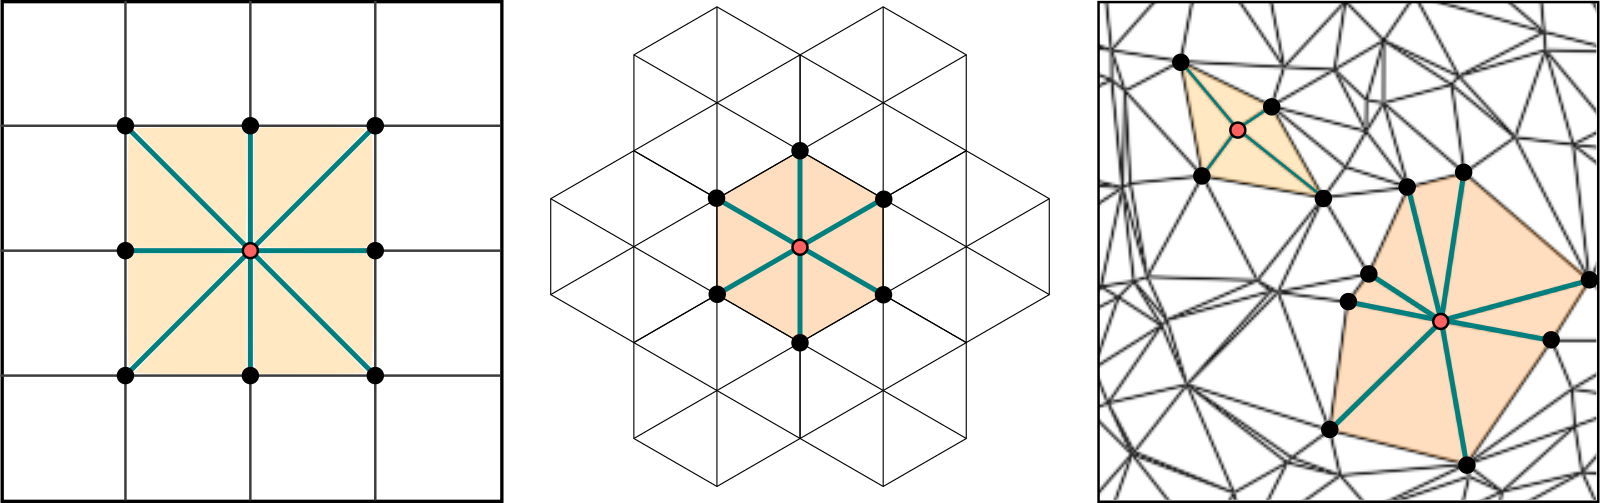
\includegraphics[width=1.0\linewidth]{figures/neighborhoods_presentation.png}
	\begin{columns}[c]
		\begin{column}{.33\textwidth}
			a regular square mesh, as in pixels of a digital image
		\end{column}
		\begin{column}{.33\textwidth}
			a regular triangle mesh, as in a hexagonal tessellation
		\end{column}
		\begin{column}{.33\textwidth}
			an irregular triangle mesh, typical of acquired \tdd{}.
		\end{column}
	\end{columns}
}

%------------------------------------------------
\frame{\frametitle{Function Values as a Scalar Field}
	\begin{columns}[c]
		\begin{column}{.75\textwidth}
			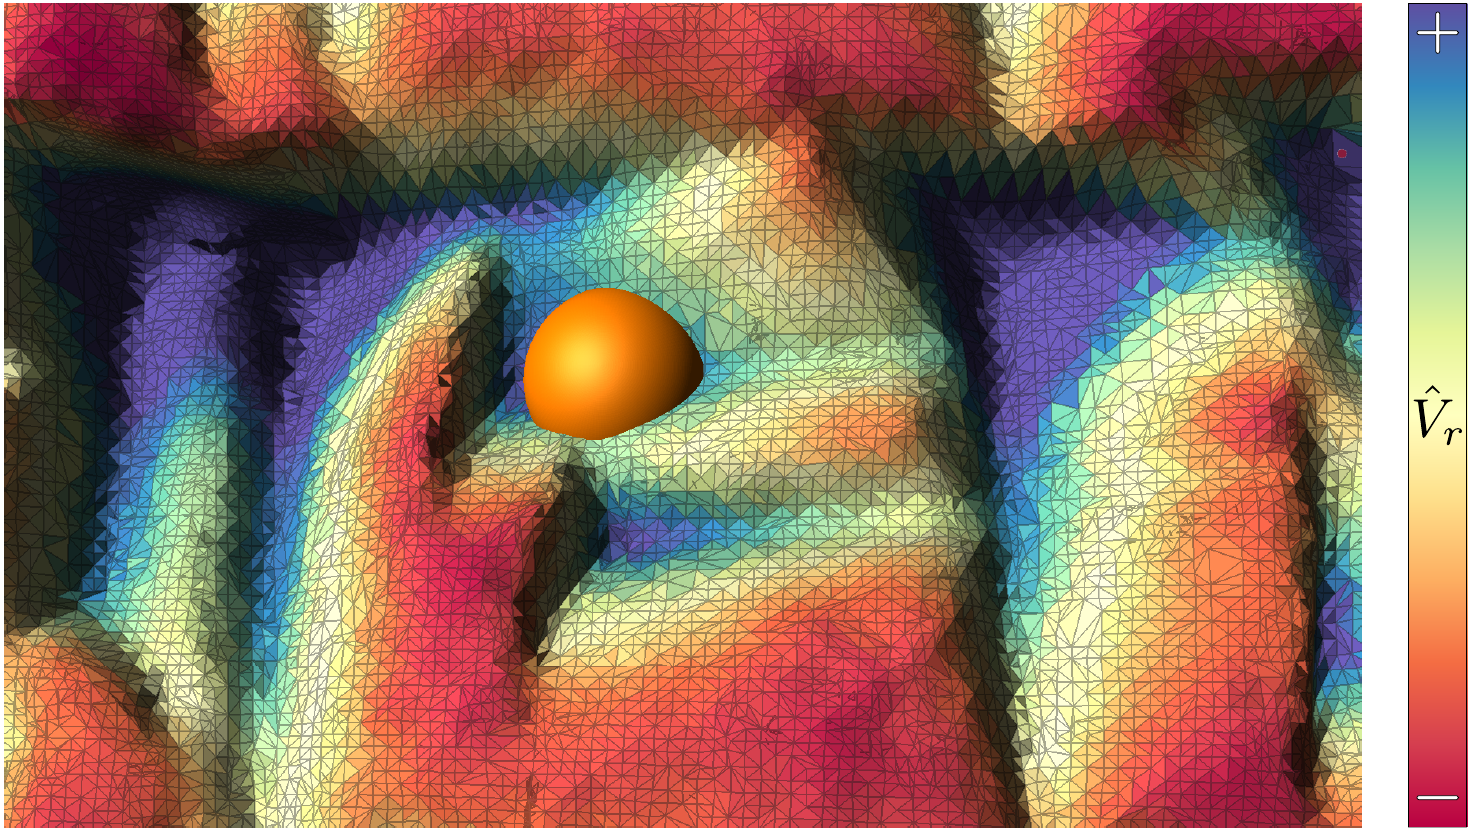
\includegraphics[width=1.0\linewidth]{figures/visualizeFunctionValues2.png}
		\end{column}
		\begin{column}{.25\textwidth}
			Visualization of the curvature of function values feature boundries, connected segments, cuneiform tablets
		\end{column}
	\end{columns}
}




%================================================
%================================================
\section{Fast One-Ring Smoothing}


%================================================
\subsection{Mathematical Foundation}

%------------------------------------------------
\frame{\frametitle{A One-Ring Neighborhood and its Geodesic Disc}
	\centering
	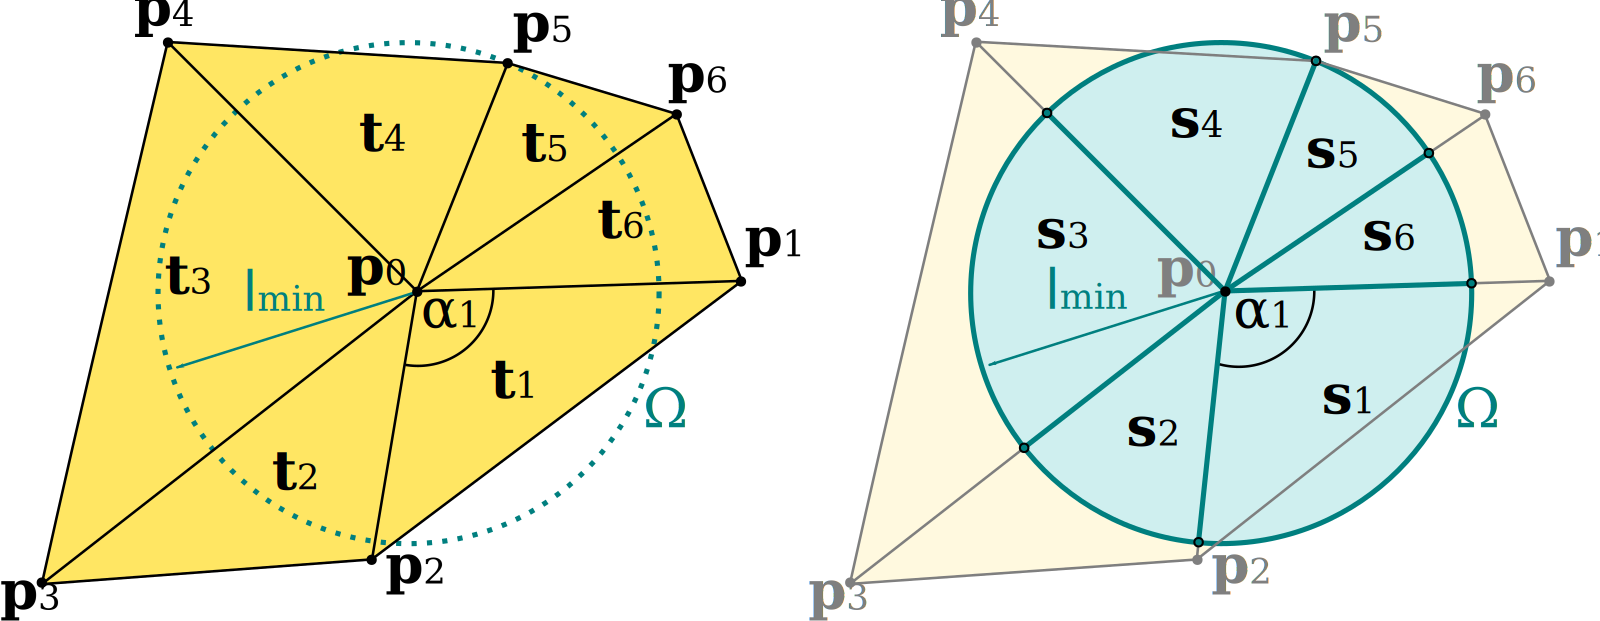
\includegraphics[width=0.8\linewidth]{figures/geodesicDisc_presentation.png}
	\begin{align*}
		\elm(\bp_0) &:= \min_{\forall \bp_i \in \bN_v}|\bp_i - \bp_0| \\
		\gelm &:= \min\left \{\elm(\bp_0) \;|\; \bp_0 \in \bM\,\right \}
	\end{align*}
}

%------------------------------------------------
\frame{\frametitle{An Enhanced View of a Circle Sector}
	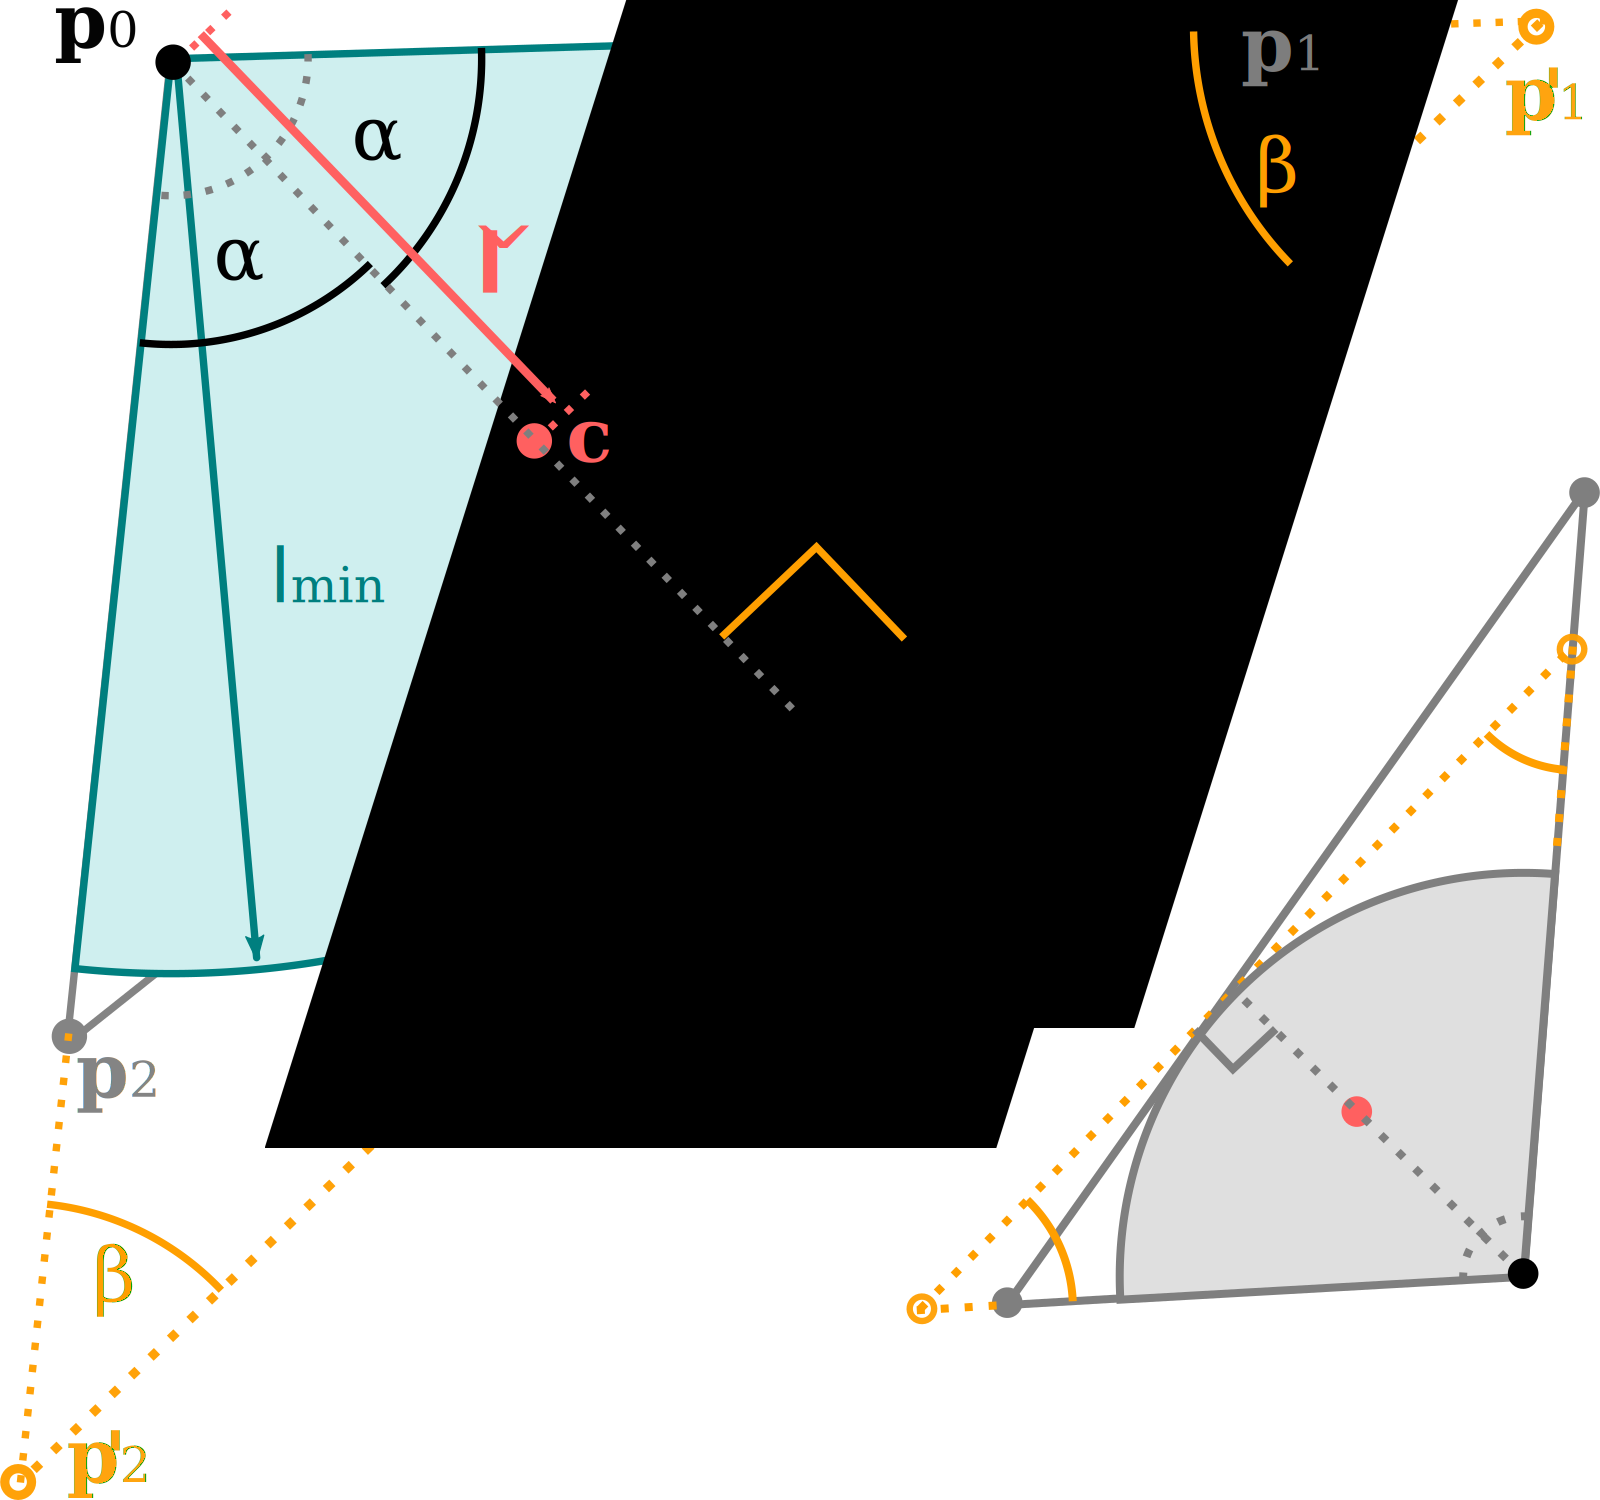
\includegraphics[width=0.5\linewidth]{figures/anglesAndCenterOfGravity_presentation.png}
}

%------------------------------------------------
\frame{\frametitle{Interpolation of Function Values toward the Center of Gravity}
	\centering
	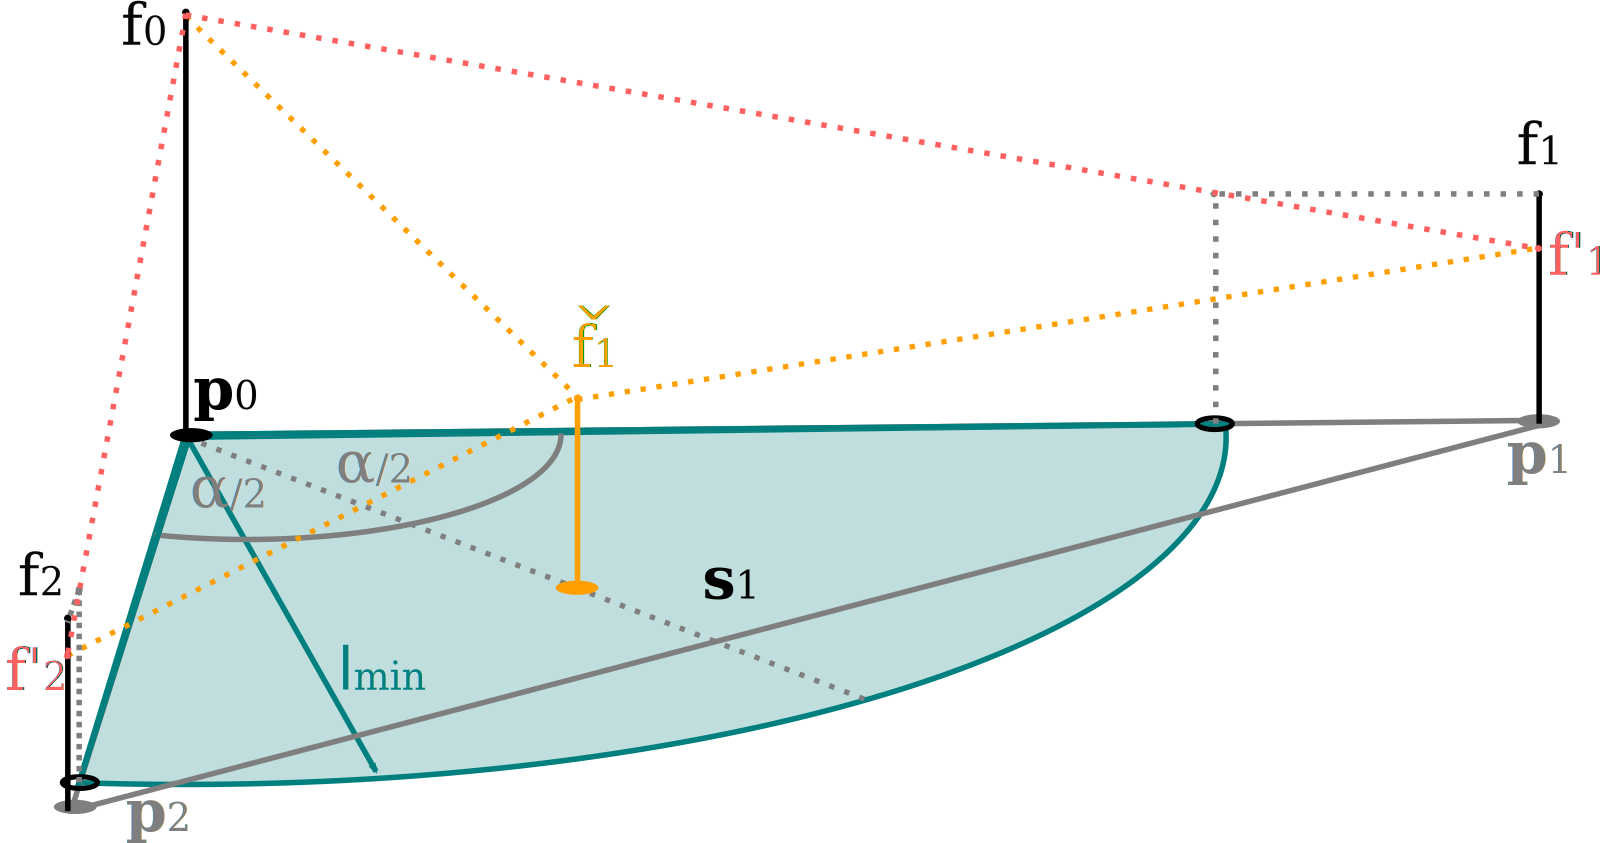
\includegraphics[width=0.9\linewidth]{figures/interpolatedFunctionValues.png}
}

%------------------------------------------------
\frame{\frametitle{Weighted Mean Function Value $f'_v$ at $\bp_v$}
	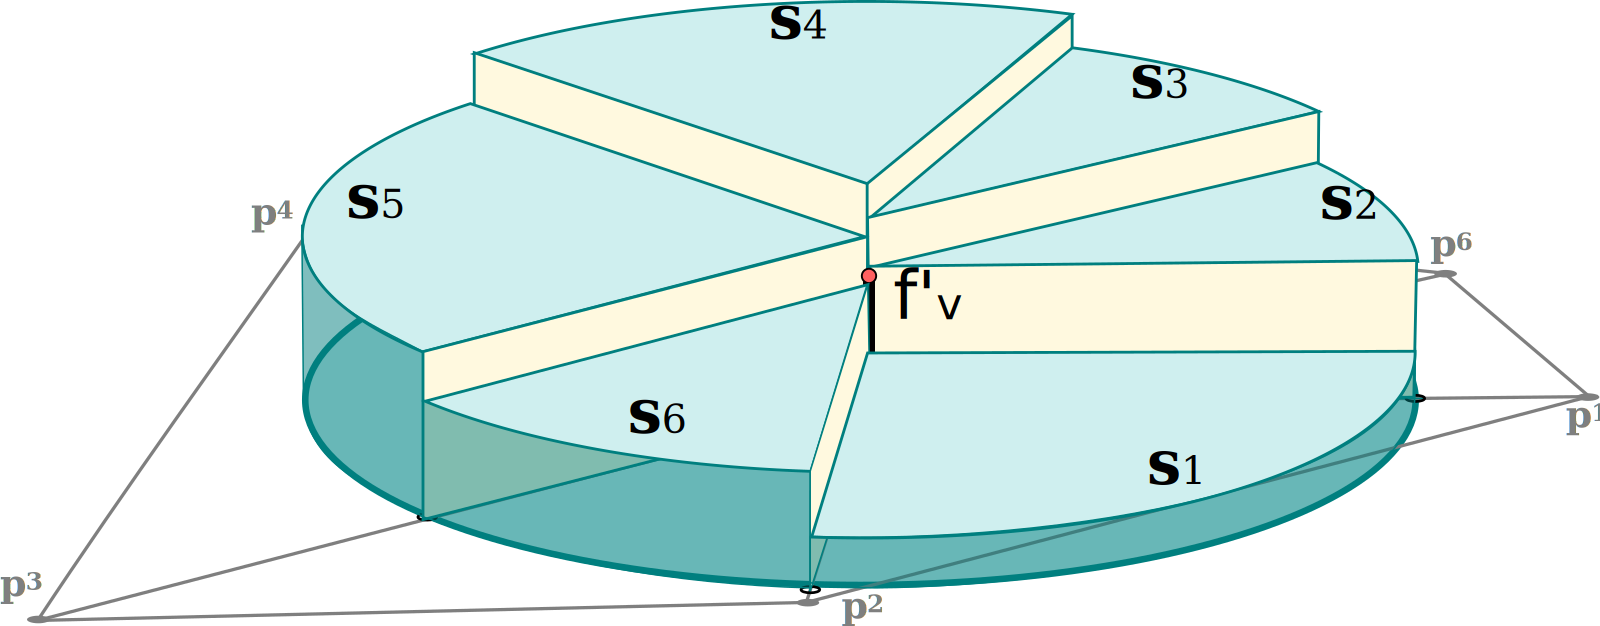
\includegraphics[width=1.0\linewidth]{figures/funcValVolumes_presentation.png}
}


%================================================
\subsection{Serial Algorithm}

%------------------------------------------------
\frame{\frametitle{Union Operations as Performed in Build Neighborhoods}
	\begin{columns}[t]
		\begin{column}{.6\textwidth}
			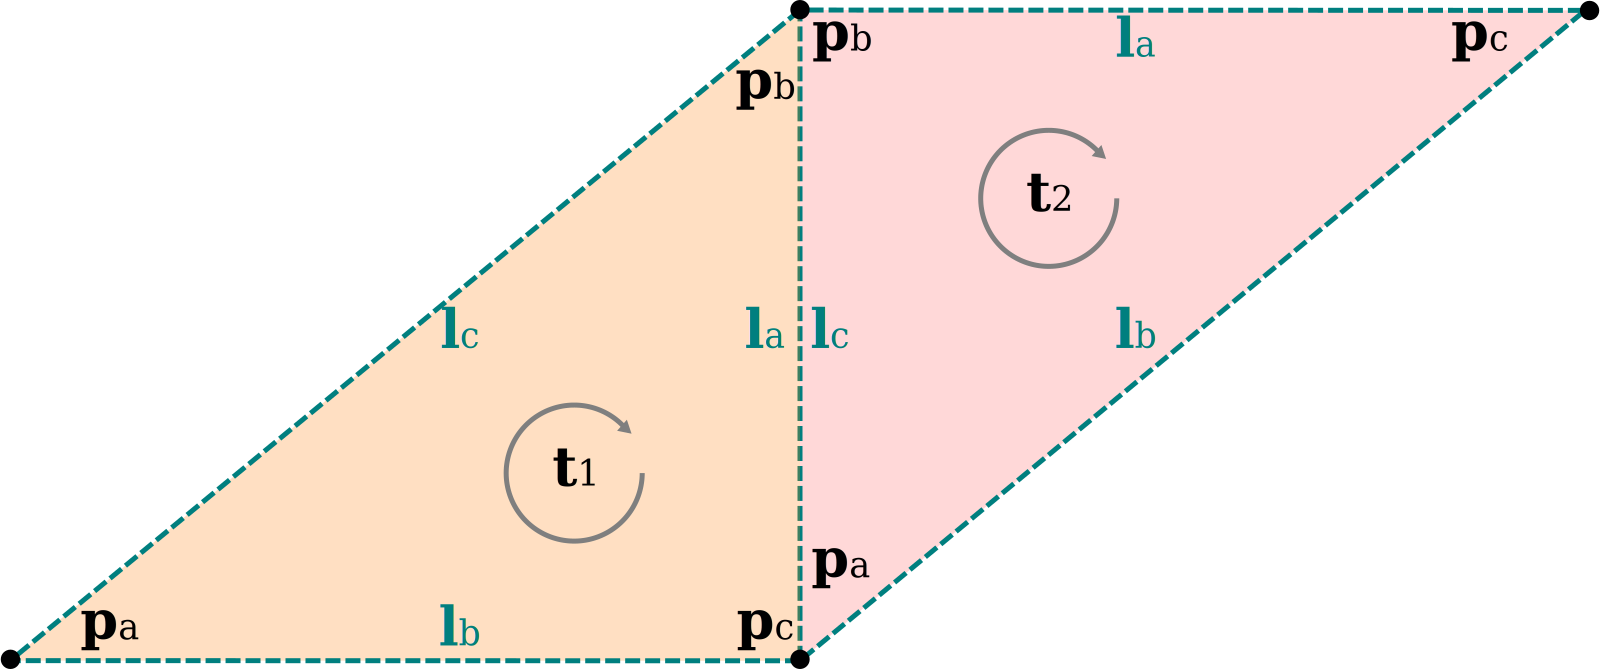
\includegraphics[width=1.0\linewidth]{figures/triangularFaces.png}
		\end{column}
		\hspace*{-1.5cm}
		\begin{column}{.6\textwidth}
			\includestandalone[width=1.0\linewidth]{figures/tikz/unionsOfSimpleBuildNeighborhoods}
		\end{column}
	\end{columns}

	\begin{columns}[t]
		\begin{column}{.5\textwidth}
			\begin{algorithm}[H]
				\DontPrintSemicolon
				\SetKwFor{For}{for}{:}{}
				\begin{block}{}
				\nl		\For{$\bt \in \bT$}{
				\nl			\ProgSty{union($\bN$, $\bp_a$, $\bp_b$, $\bp_c$)}\;
				\nl			\ProgSty{union($\bN$, $\bp_b$, $\bp_a$, $\bp_c$)}\;
				\nl			\ProgSty{union($\bN$, $\bp_c$, $\bp_a$, $\bp_b$)}\;
						}
				\end{block}
			\end{algorithm}
		\end{column}
		\begin{column}{.5\textwidth}
			\begin{algorithm}[H]
				\DontPrintSemicolon
				\SetKwFor{For}{for}{:}{}
				\SetKwProg{Func}{Function}{}{}
				\begin{block}{}
				\nl	\Func{union($\bN$, $a$, $b$, $c$)}{
				\nl		$\bN_a \leftarrow \bN_a \cup \{b,\,c\}$\;
					}
				\end{block}
			\end{algorithm}
		\end{column}
	\end{columns}
}

%------------------------------------------------
\frame{\frametitle{Serial Algorithm for Calculating Edge Lengths}
\begin{algorithm}[H]
	\SetAlgoSkip{}
	\DontPrintSemicolon
	\SetCommentSty{small}
	\SetKwFor{For}{for}{:}{}
	\SetKwProg{Func}{Function}{}{}
	\SetKwInOut{Input}{Input}\SetKwInOut{Output}{Output}

	\only<1>{
	\begin{block}{}%Part (1 of 1)}
		\Input{the set of all points $\bP$, \\
			the set of discovered neighborhoods $\bN$}
		\Output{the set of pre-calculated edge lengths $\bE$, \\
			the minimum edge length of the mesh $\gelm$}

		\bigskip
	\nl	\Func{serialCalculateEdgeLengths($\bP$, $\bN$)}{
	\nl		\For{$\bp_v \in \bP$}{
	\nl			\For{$\bp_i \in \bN_v$}{
					\linespread{1.5}\selectfont
	\nl				$\bE_{\sv{i}} \leftarrow |\bp_i - \bp_v|$\tcc*[r]{This is $\ellstar$}
	\nl				$\gelm \leftarrow \min\left \{\gelm,\,\bE_{\sv{i}}\right \}$\;
				}
			}
		}
	\end{block}
	}
\end{algorithm}
}

%------------------------------------------------
\frame{\frametitle{Serial Algorithm for Convolving the Filter}
	\vspace*{-8mm}
	\begin{columns}
		\begin{column}[t]{.35\textwidth}
			\begin{block}{}
				{\fontsize{4.2}{4.2}\selectfont
					\begin{algorithm}[H]
						\DontPrintSemicolon
						\SetCommentSty{small}
						\SetKwFor{For}{for}{:}{}
						\SetKwProg{Func}{Function}{}{}
						\SetKwProg{Cont}{}{}{}
						\SetKwInOut{Input}{Input}\SetKwInOut{Output}{Output}
						\Input{the set of all points $\bP$, \\
							the set of discovered neighborhoods $\bN$, \\
							the set of pre-calculated edge lengths $\bE$, \\
							the minimum edge length of the mesh $\gelm$, \\
							the set of function values $\bF$, \\
							the user-defined number of convolutions $\tau$}
						\Output{the set of one-ring \wmfv{s} $\bF'$}

						\medskip
						\linespread{1.2}\selectfont
					\nl	\Func{serialConvolveFilter($\bP$, $\bN$, $\bE$, $\gelm$, $\bF$, $\tau$)}{
					\nl		\For{$t\leftarrow 1\;\KwTo\;\tau$}{
					\nl			\For{$\bp_v \in \bP$}{
					\nl				\For{$\bp_i \in \bN_v$}{
										\linespread{1.5}\selectfont
					\nl					$\kern-0.5pt\alpha \leftarrow cos^{-1} \kern-6pt\left (\frac{\bE_c^2\,+\,\bE_b^2\,-\,\bE_a^2}{2\,\cdot\,\bE_c\,\cdot\,\bE_b}\right )$\;
										\linespread{1.2}\selectfont
					\nl					$\kern0.00pt\beta \leftarrow (\pi - \alpha)\mathbin{/}2$\;
					\nl					$\kern-1.5ptA \leftarrow \Big(\gelm\,\Big)^2\kern-4pt\cdot\alpha\mathbin{/}2$\;
					\nl					$\kern1.00pt\check{\ell} \leftarrow \big(4\cdot\gelm\cdot\sin(\alpha\mathbin{/}2)\big)\mathbin{/}3\,\alpha$\;
					\nl					$\kern1.00pt\zeta \leftarrow \gelm\mathbin{/}\sin(\beta)$\;
					\nl					\For{$j \in {1,2}$}{\label{algSCFjloop}
					\nl						$\tilde{\ell}_j \leftarrow \zeta\mathbin{/}\bE_j$\;
					\nl						$f'_j \leftarrow f_0\cdot(1 - \tilde{\ell}_j) + f_j\cdot\tilde{\ell}_j$\;
										}
					\nl					$\check{f} \leftarrow f_0\cdot(1 - \check{\ell}) + \big((f'_1 + f'_2)\cdot\check{\ell}\big)\mathbin{/}2$\;
					\nl					$\kern-2.0pt\tilde{f}_v \leftarrow \tilde{f}_v + A\cdot\check{f}$\;
					\nl					$\kern-4.0pt\tilde{A}_v \leftarrow \tilde{A}_v + A$\;
									}
					\nl				$f'_v \leftarrow \tilde{f}_v\mathbin{/}\tilde{A}_v$\;
								}
					\nl		$\bF' \leftarrow \left \{f'_1,\ldots,\,f'_{|\bP|}\right \}$\;
					\nl 	$\bF \leftarrow \bF'$\;
							}
						}
					\end{algorithm}
				}
			\end{block}
		\end{column}
		\begin{column}[t]{.65\textwidth}				
			\only<1>{
				\begin{block}{Part (1 of 3)}
					\begin{algorithm}[H]
						\DontPrintSemicolon
						\SetCommentSty{small}
						\SetKwFor{For}{for}{:}{}
						\SetKwProg{Func}{Function}{}{}
						\SetKwProg{Cont}{}{}{}
						\SetKwInOut{Input}{Input}\SetKwInOut{Output}{Output}
						\Input{the set of all points $\bP$, \\
							the set of discovered neighborhoods $\bN$, \\
							the set of pre-calculated edge lengths $\bE$, \\
							the minimum edge length of the mesh $\gelm$, \\
							the set of function values $\bF$, \\
							the user-defined number of convolutions $\tau$}
						\Output{the set of one-ring \wmfv{s} $\bF'$}
					\end{algorithm}
				\end{block}
			}\only<2>{
				\begin{block}{Part (2 of 3)}
					\begin{algorithm}[H]
						\SetAlgoLined
						\DontPrintSemicolon
						\SetCommentSty{small}
						\SetKwFor{For}{for}{:}{}
						\SetKwProg{Func}{Function}{}{}
						\SetKwProg{Cont}{}{}{}
						\setcounter{AlgoLine}{0}
					\nl	\Func{serialConvolveFilter($\bP$, $\bN$, $\bE$, $\gelm$, $\bF$, $\tau$)}{
					\nl		\For{$t\leftarrow 1\;\KwTo\;\tau$}{
					\nl			\For{$\bp_v \in \bP$}{
					\nl				\For{$\bp_i \in \bN_v$}{
										\vspace*{1.5\baselineskip}
										\ldots
										\vspace*{1.5\baselineskip}
									}
						\setcounter{AlgoLine}{15}
					\nl				$f'_v \leftarrow \tilde{f}_v\mathbin{/}\tilde{A}_v$\;
								}
					\nl		$\bF' \leftarrow \left \{f'_1,\ldots,\,f'_{|\bP|}\right \}$\;
					\nl 	$\bF \leftarrow \bF'$\;
							}
						}
					\end{algorithm}
				\end{block}
			}\only<3>{
				\begin{block}{Part (3 of 3)}
					{\fontsize{9}{9.5}\selectfont
					\begin{algorithm}[H]
						\SetAlgoLined
						\DontPrintSemicolon
						\SetCommentSty{small}
						\SetKwFor{For}{for}{:}{}
						\SetKwProg{Func}{Function}{}{}
						\SetKwProg{Cont}{}{}{}
						\setcounter{AlgoLine}{7}
						\vspace*{-1\baselineskip}
						\Cont{}{
							\vspace*{-1\baselineskip}
							\Cont{}{
								\vspace*{-1\baselineskip}
								\Cont{}{
									\vspace*{-1\baselineskip}
									\Cont{}{					
										\linespread{1.5}\selectfont
					\nl					$\kern-0.5pt\alpha \leftarrow cos^{-1} \kern-6pt\left (\frac{\bE_c^2\,+\,\bE_b^2\,-\,\bE_a^2}{2\,\cdot\,\bE_c\,\cdot\,\bE_b}\right )$\;
										\linespread{1.2}\selectfont
					\nl					$\kern0.00pt\beta \leftarrow (\pi - \alpha)\mathbin{/}2$\;
					\nl					$\kern-1.5ptA \leftarrow \Big(\gelm\,\Big)^2\kern-4pt\cdot\alpha\mathbin{/}2$\;
					\nl					$\kern1.00pt\check{\ell} \leftarrow \big(4\cdot\gelm\cdot\sin(\alpha\mathbin{/}2)\big)\mathbin{/}3\,\alpha$\;
					\nl					$\kern1.00pt\zeta \leftarrow \gelm\mathbin{/}\sin(\beta)$\;
					\nl					\For{$j \in {1,2}$}{\label{algSCFjloop}
					\nl						$\tilde{\ell}_j \leftarrow \zeta\mathbin{/}\bE_j$\;
					\nl						$f'_j \leftarrow f_0\cdot(1 - \tilde{\ell}_j) + f_j\cdot\tilde{\ell}_j$\;
										}
					\nl					$\check{f} \leftarrow f_0\cdot(1 - \check{\ell}) + \big((f'_1 + f'_2)\cdot\check{\ell}\big)\mathbin{/}2$\;
					\nl					$\kern-2.0pt\tilde{f}_v \leftarrow \tilde{f}_v + A\cdot\check{f}$\;
					\nl					$\kern-4.0pt\tilde{A}_v \leftarrow \tilde{A}_v + A$\;
									}
								}
							}
						}
					\end{algorithm}
					}
				\end{block}
			}
		\end{column}
	\end{columns}
	\begin{tikzpicture}[overlay, remember picture]
		\draw<1>[unirot,ultra thick,rounded corners] (-8mm, 64mm) rectangle (46mm, 50mm);
		\draw<2>[unirot,ultra thick,rounded corners] (-8mm, 50mm) rectangle (46mm, 41mm);
		\draw<2>[unirot,ultra thick,rounded corners] (-8mm, 15mm) rectangle (46mm,  2mm);
		\draw<3>[unirot,ultra thick,rounded corners] (-8mm, 43mm) rectangle (46mm, 14mm);
	\end{tikzpicture}
}


%================================================
\subsection{Data Dependencies}

%------------------------------------------------
\frame{\frametitle{Data Dependencies in Serial Algorithm Build Neighborhoods}
	\centering
	\includestandalone[width=0.75\textwidth]{figures/tikz/sabnDataDependencies}
}

%------------------------------------------------
\frame{\frametitle{Data Dependencies in Serial Algorithm Calculate Edge Lengths}
	\centering
	\includestandalone[width=0.85\textwidth]{figures/tikz/sacelDataDependencies}
}

%------------------------------------------------
\frame{\frametitle{Data Dependencies in Serial Algorithm Convolve Filter}
	\centering
	\includestandalone[width=0.5\textwidth]{figures/tikz/sacfDataDependencies}
} 


%================================================
\subsection{Parallel Algorithm}

%------------------------------------------------
\frame{\frametitle{Parallel Alg. 1}

}

%------------------------------------------------
\frame{\frametitle{Parallel Algorithm for Calculating Edge Lengths}
\begin{algorithm}[H]
	\SetAlgoSkip{}
	\DontPrintSemicolon
	\SetCommentSty{small}
	\SetKwFor{For}{for}{:}{}
	\SetKwProg{Func}{Function}{}{}
	\SetKwInOut{Input}{Input}\SetKwInOut{Output}{Output}

	\only<1>{
	\begin{block}{}%Part (1 of 1)}
		\Input{the set of all points $\bP$, \\
			the set of discovered neighborhoods $\bN$}
		\Output{the set of pre-calculated edge lengths $\bE$, \\
			the minimum edge length of the mesh $\gelm$}

		\bigskip
	\nl	\Func{serialCalculateEdgeLengths($\bP$, $\bN$)}{
	\nl		\For{$\bp_v \in \bP$}{
	\nl			\For{$\bp_i \in \bN_v$}{
					\linespread{1.5}\selectfont
	\nl				$\bE_{\sv{i}} \leftarrow |\bp_i - \bp_v|$\tcc*[r]{This is $\ellstar$}
	\nl				$\gelm \leftarrow \min\left \{\gelm,\,\bE_{\sv{i}}\right \}$\;
				}
			}
		}
	\end{block}
	}
\end{algorithm}
}

%------------------------------------------------
\frame{\frametitle{Parallel Algorithm for Convolving the Filter}
	\vspace*{-8mm}
	\begin{columns}
		\begin{column}[t]{.35\textwidth}
			\begin{block}{}
				{\fontsize{4.2}{4.2}\selectfont
					\begin{algorithm}[H]
						\DontPrintSemicolon
						\SetCommentSty{small}
						\SetKwFor{For}{for}{:}{}
						\SetKwProg{Func}{Function}{}{}
						\SetKwProg{Cont}{}{}{}
						\SetKwInOut{Input}{Input}\SetKwInOut{Output}{Output}
						\Input{the set of all points $\bP$, \\
							the set of discovered neighborhoods $\bN$, \\
							the set of pre-calculated edge lengths $\bE$, \\
							the minimum edge length of the mesh $\gelm$, \\
							the set of function values $\bF$, \\
							the user-defined number of convolutions $\tau$}
						\Output{the set of one-ring \wmfv{s} $\bF'$}

						\medskip
						\linespread{1.2}\selectfont
					\nl	\Func{serialConvolveFilter($\bP$, $\bN$, $\bE$, $\gelm$, $\bF$, $\tau$)}{
					\nl		\For{$t\leftarrow 1\;\KwTo\;\tau$}{
					\nl			\For{$\bp_v \in \bP$}{
					\nl				\For{$\bp_i \in \bN_v$}{
										\linespread{1.5}\selectfont
					\nl					$\kern-0.5pt\alpha \leftarrow cos^{-1} \kern-6pt\left (\frac{\bE_c^2\,+\,\bE_b^2\,-\,\bE_a^2}{2\,\cdot\,\bE_c\,\cdot\,\bE_b}\right )$\;
										\linespread{1.2}\selectfont
					\nl					$\kern0.00pt\beta \leftarrow (\pi - \alpha)\mathbin{/}2$\;
					\nl					$\kern-1.5ptA \leftarrow \Big(\gelm\,\Big)^2\kern-4pt\cdot\alpha\mathbin{/}2$\;
					\nl					$\kern1.00pt\check{\ell} \leftarrow \big(4\cdot\gelm\cdot\sin(\alpha\mathbin{/}2)\big)\mathbin{/}3\,\alpha$\;
					\nl					$\kern1.00pt\zeta \leftarrow \gelm\mathbin{/}\sin(\beta)$\;
					\nl					\For{$j \in {1,2}$}{\label{algSCFjloop}
					\nl						$\tilde{\ell}_j \leftarrow \zeta\mathbin{/}\bE_j$\;
					\nl						$f'_j \leftarrow f_0\cdot(1 - \tilde{\ell}_j) + f_j\cdot\tilde{\ell}_j$\;
										}
					\nl					$\check{f} \leftarrow f_0\cdot(1 - \check{\ell}) + \big((f'_1 + f'_2)\cdot\check{\ell}\big)\mathbin{/}2$\;
					\nl					$\kern-2.0pt\tilde{f}_v \leftarrow \tilde{f}_v + A\cdot\check{f}$\;
					\nl					$\kern-4.0pt\tilde{A}_v \leftarrow \tilde{A}_v + A$\;
									}
					\nl				$f'_v \leftarrow \tilde{f}_v\mathbin{/}\tilde{A}_v$\;
								}
					\nl		$\bF' \leftarrow \left \{f'_1,\ldots,\,f'_{|\bP|}\right \}$\;
					\nl 	$\bF \leftarrow \bF'$\;
							}
						}
					\end{algorithm}
				}
			\end{block}
		\end{column}
		\begin{column}[t]{.65\textwidth}				
			\only<1>{
				\begin{block}{Part (1 of 3)}
					\begin{algorithm}[H]
						\DontPrintSemicolon
						\SetCommentSty{small}
						\SetKwFor{For}{for}{:}{}
						\SetKwProg{Func}{Function}{}{}
						\SetKwProg{Cont}{}{}{}
						\SetKwInOut{Input}{Input}\SetKwInOut{Output}{Output}
						\Input{the set of all points $\bP$, \\
							the set of discovered neighborhoods $\bN$, \\
							the set of pre-calculated edge lengths $\bE$, \\
							the minimum edge length of the mesh $\gelm$, \\
							the set of function values $\bF$, \\
							the user-defined number of convolutions $\tau$}
						\Output{the set of one-ring \wmfv{s} $\bF'$}
					\end{algorithm}
				\end{block}
			}\only<2>{
				\begin{block}{Part (2 of 3)}
					\begin{algorithm}[H]
						\SetAlgoLined
						\DontPrintSemicolon
						\SetCommentSty{small}
						\SetKwFor{For}{for}{:}{}
						\SetKwProg{Func}{Function}{}{}
						\SetKwProg{Cont}{}{}{}
						\setcounter{AlgoLine}{0}
					\nl	\Func{serialConvolveFilter($\bP$, $\bN$, $\bE$, $\gelm$, $\bF$, $\tau$)}{
					\nl		\For{$t\leftarrow 1\;\KwTo\;\tau$}{
					\nl			\For{$\bp_v \in \bP$}{
					\nl				\For{$\bp_i \in \bN_v$}{
										\vspace*{1.5\baselineskip}
										\ldots
										\vspace*{1.5\baselineskip}
									}
						\setcounter{AlgoLine}{15}
					\nl				$f'_v \leftarrow \tilde{f}_v\mathbin{/}\tilde{A}_v$\;
								}
					\nl		$\bF' \leftarrow \left \{f'_1,\ldots,\,f'_{|\bP|}\right \}$\;
					\nl 	$\bF \leftarrow \bF'$\;
							}
						}
					\end{algorithm}
				\end{block}
			}\only<3>{
				\begin{block}{Part (3 of 3)}
					{\fontsize{9}{9.5}\selectfont
					\begin{algorithm}[H]
						\SetAlgoLined
						\DontPrintSemicolon
						\SetCommentSty{small}
						\SetKwFor{For}{for}{:}{}
						\SetKwProg{Func}{Function}{}{}
						\SetKwProg{Cont}{}{}{}
						\setcounter{AlgoLine}{7}
						\vspace*{-1\baselineskip}
						\Cont{}{
							\vspace*{-1\baselineskip}
							\Cont{}{
								\vspace*{-1\baselineskip}
								\Cont{}{
									\vspace*{-1\baselineskip}
									\Cont{}{					
										\linespread{1.5}\selectfont
					\nl					$\kern-0.5pt\alpha \leftarrow cos^{-1} \kern-6pt\left (\frac{\bE_c^2\,+\,\bE_b^2\,-\,\bE_a^2}{2\,\cdot\,\bE_c\,\cdot\,\bE_b}\right )$\;
										\linespread{1.2}\selectfont
					\nl					$\kern0.00pt\beta \leftarrow (\pi - \alpha)\mathbin{/}2$\;
					\nl					$\kern-1.5ptA \leftarrow \Big(\gelm\,\Big)^2\kern-4pt\cdot\alpha\mathbin{/}2$\;
					\nl					$\kern1.00pt\check{\ell} \leftarrow \big(4\cdot\gelm\cdot\sin(\alpha\mathbin{/}2)\big)\mathbin{/}3\,\alpha$\;
					\nl					$\kern1.00pt\zeta \leftarrow \gelm\mathbin{/}\sin(\beta)$\;
					\nl					\For{$j \in {1,2}$}{\label{algSCFjloop}
					\nl						$\tilde{\ell}_j \leftarrow \zeta\mathbin{/}\bE_j$\;
					\nl						$f'_j \leftarrow f_0\cdot(1 - \tilde{\ell}_j) + f_j\cdot\tilde{\ell}_j$\;
										}
					\nl					$\check{f} \leftarrow f_0\cdot(1 - \check{\ell}) + \big((f'_1 + f'_2)\cdot\check{\ell}\big)\mathbin{/}2$\;
					\nl					$\kern-2.0pt\tilde{f}_v \leftarrow \tilde{f}_v + A\cdot\check{f}$\;
					\nl					$\kern-4.0pt\tilde{A}_v \leftarrow \tilde{A}_v + A$\;
									}
								}
							}
						}
					\end{algorithm}
					}
				\end{block}
			}
		\end{column}
	\end{columns}
	\begin{tikzpicture}[overlay, remember picture]
		\draw<1>[unirot,ultra thick,rounded corners] (-8mm, 64mm) rectangle (46mm, 50mm);
		\draw<2>[unirot,ultra thick,rounded corners] (-8mm, 50mm) rectangle (46mm, 41mm);
		\draw<2>[unirot,ultra thick,rounded corners] (-8mm, 15mm) rectangle (46mm,  2mm);
		\draw<3>[unirot,ultra thick,rounded corners] (-8mm, 43mm) rectangle (46mm, 14mm);
	\end{tikzpicture}
}




%================================================
%================================================
\section{Experiments \& Evaluation}


%================================================
\subsection{Filter Response On Synthetic Data}

%------------------------------------------------
\frame{\frametitle{Bisected-Square Tessellations}
	\begin{figure}[ht]
	\begin{subfigure}[b]{0.32\linewidth}
		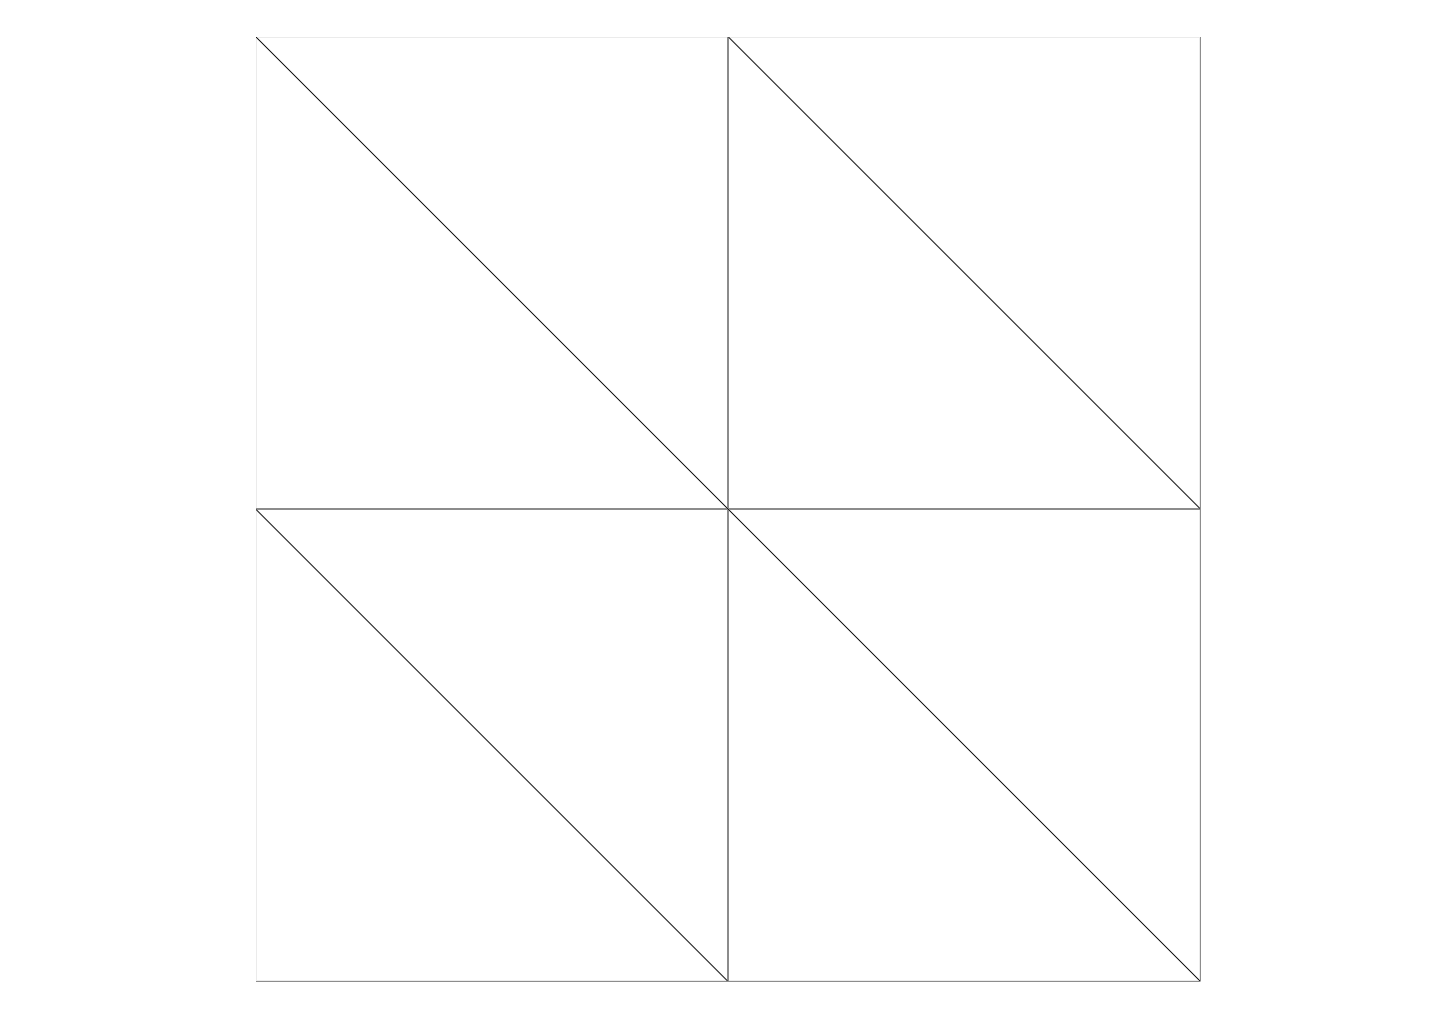
\includegraphics[width=\linewidth]
		{data/synthetic_meshes/square_tesselation_2tri_Dirac_delta_1_v9_f8_wireframe.png}
		\caption{$r=1$, wireframe}\label{fig:sq2.a}
	\end{subfigure}
	\begin{subfigure}[b]{0.32\linewidth}
		
\includegraphics[width=\linewidth]
		{data/synthetic_meshes/square_tesselation_2tri_Dirac_delta_1_v9_f8_funcvals_0iter_crop.png}
		\caption{$r=1$, $c=0$}\label{fig:sq2.b}
	\end{subfigure}
	\begin{subfigure}[b]{0.32\linewidth}
		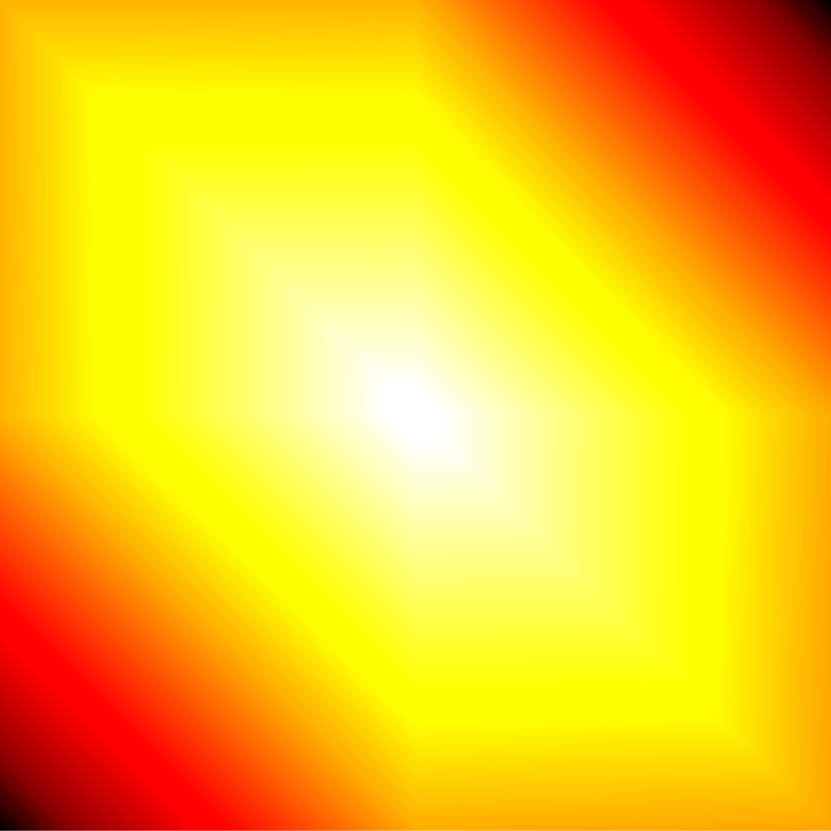
\includegraphics[width=\linewidth]
		{data/synthetic_meshes/square_tesselation_2tri_Dirac_delta_1_v9_f8_funcvals_1iter_crop.png}
		\caption{$r=1$, $c=1$}\label{fig:sq2.c}
	\end{subfigure}

	\bigskip
	\begin{subfigure}[b]{0.32\linewidth}
		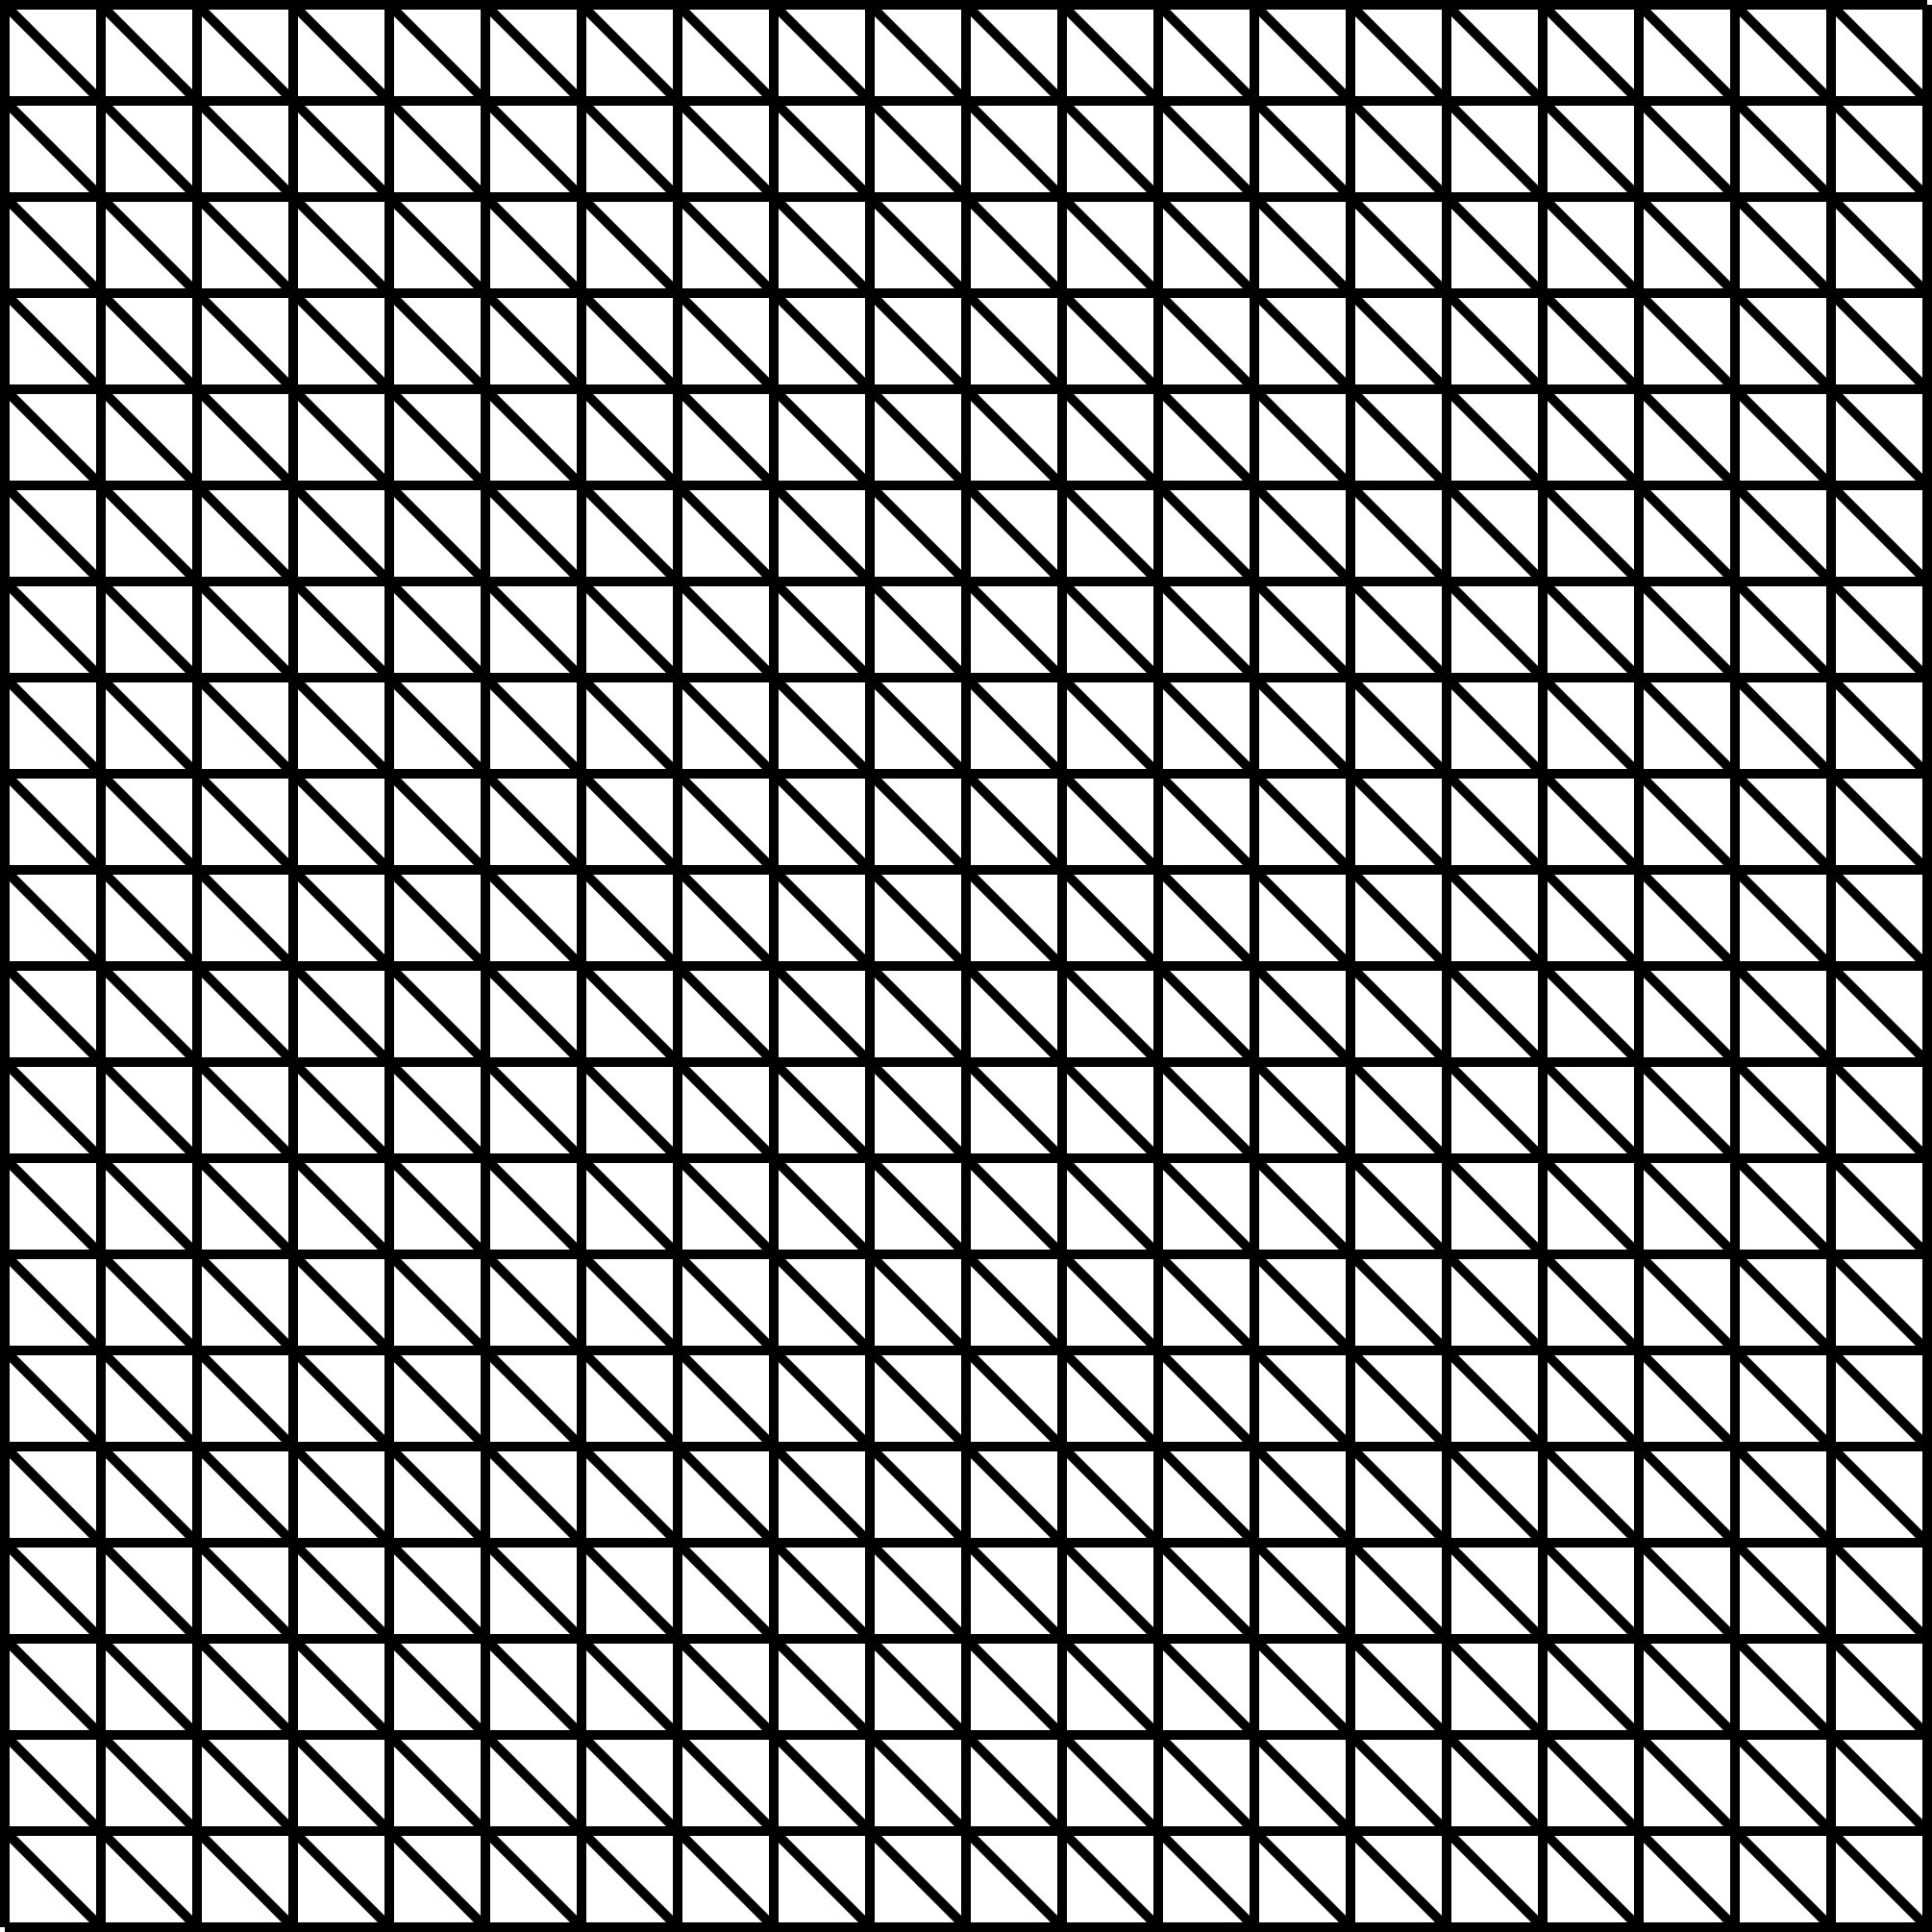
\includegraphics[width=\linewidth]
		{data/synthetic_meshes/square_tesselation_2tri_Dirac_delta_10_v441_f800_wireframe.png}
		\caption{$r=10$, wireframe}\label{fig:sq2.d}
	\end{subfigure}
	\begin{subfigure}[b]{0.32\linewidth}
		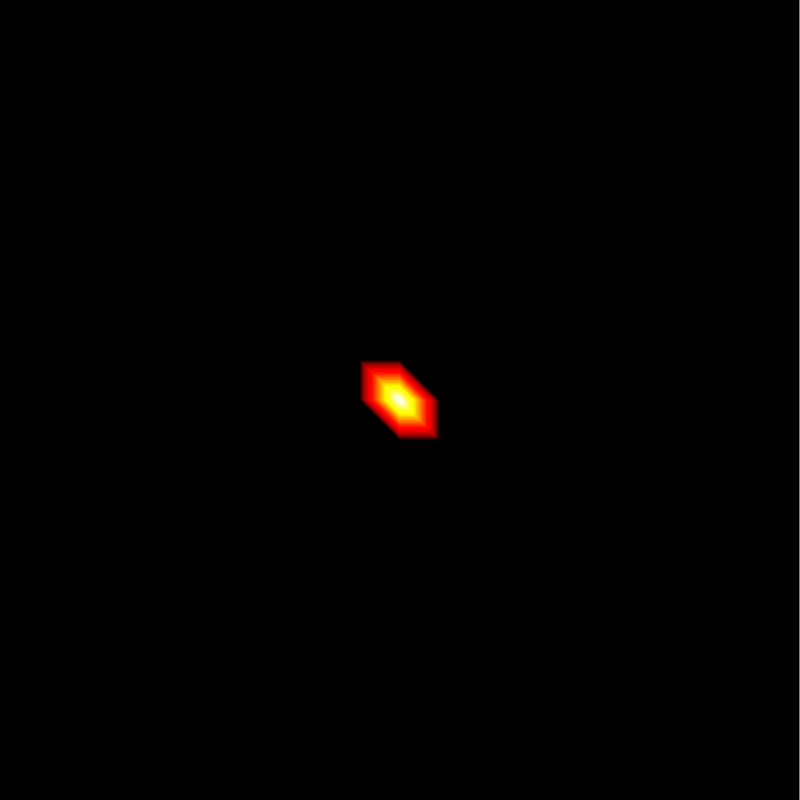
\includegraphics[width=\linewidth]
		{data/synthetic_meshes/square_tesselation_2tri_Dirac_delta_10_v441_f800_funcvals_0iter.png}
		\caption{$r=10$, $c=0$}\label{fig:sq2.e}
	\end{subfigure}
	\begin{subfigure}[b]{0.32\linewidth}
		
\includegraphics[width=\linewidth]
		{data/synthetic_meshes/square_tesselation_2tri_Dirac_delta_10_v441_f800_funcvals_100iter.png}
		\caption{$r=10$, $c=100$}\label{fig:sq2.f}
	\end{subfigure}
	\caption[Six views, comparing two differently sized of bisected square tessellations]{Comparison of two differently sized bisected square tessellations, generated with parameters $r$ set to 1 and 10: (a) $r=1$ in wireframe (b) $r=1$ colored by function value before convolving the filter (c) $r=1$ colored by function value after convolving the filter once (d) $r=10$ in wireframe (e) $r=10$ colored by function value before convoving the filter (f) $r=10$ colored by function value after convolving the filter 100 times.}
	\label{fig:sq2}
\end{figure}

}

%------------------------------------------------
\frame{\frametitle{Quadrisected-Square Tessellations}
	\begin{figure}[ht]
	\begin{subfigure}[b]{0.32\linewidth}
		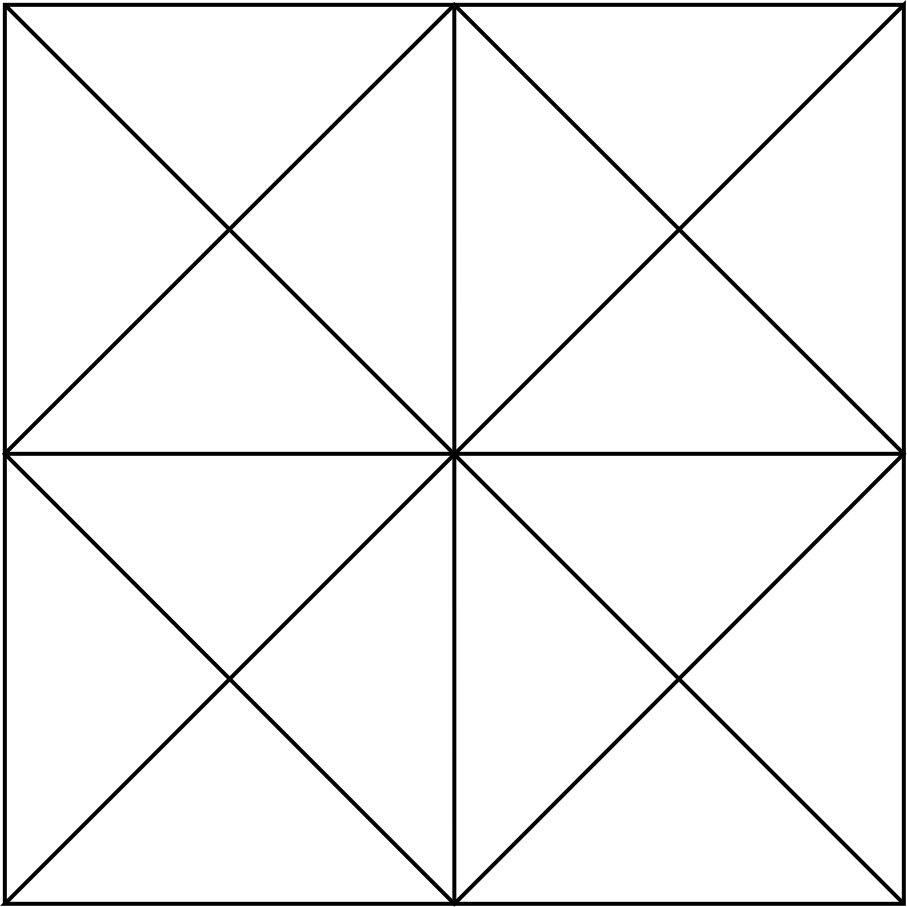
\includegraphics[width=\linewidth]
		{data/synthetic_meshes/square_tesselation_4tri_Dirac_delta_1_v13_f16_wireframe.png}
		\caption{$r=1$, wireframe}\label{fig:sq2.a}
	\end{subfigure}
	\begin{subfigure}[b]{0.32\linewidth}
		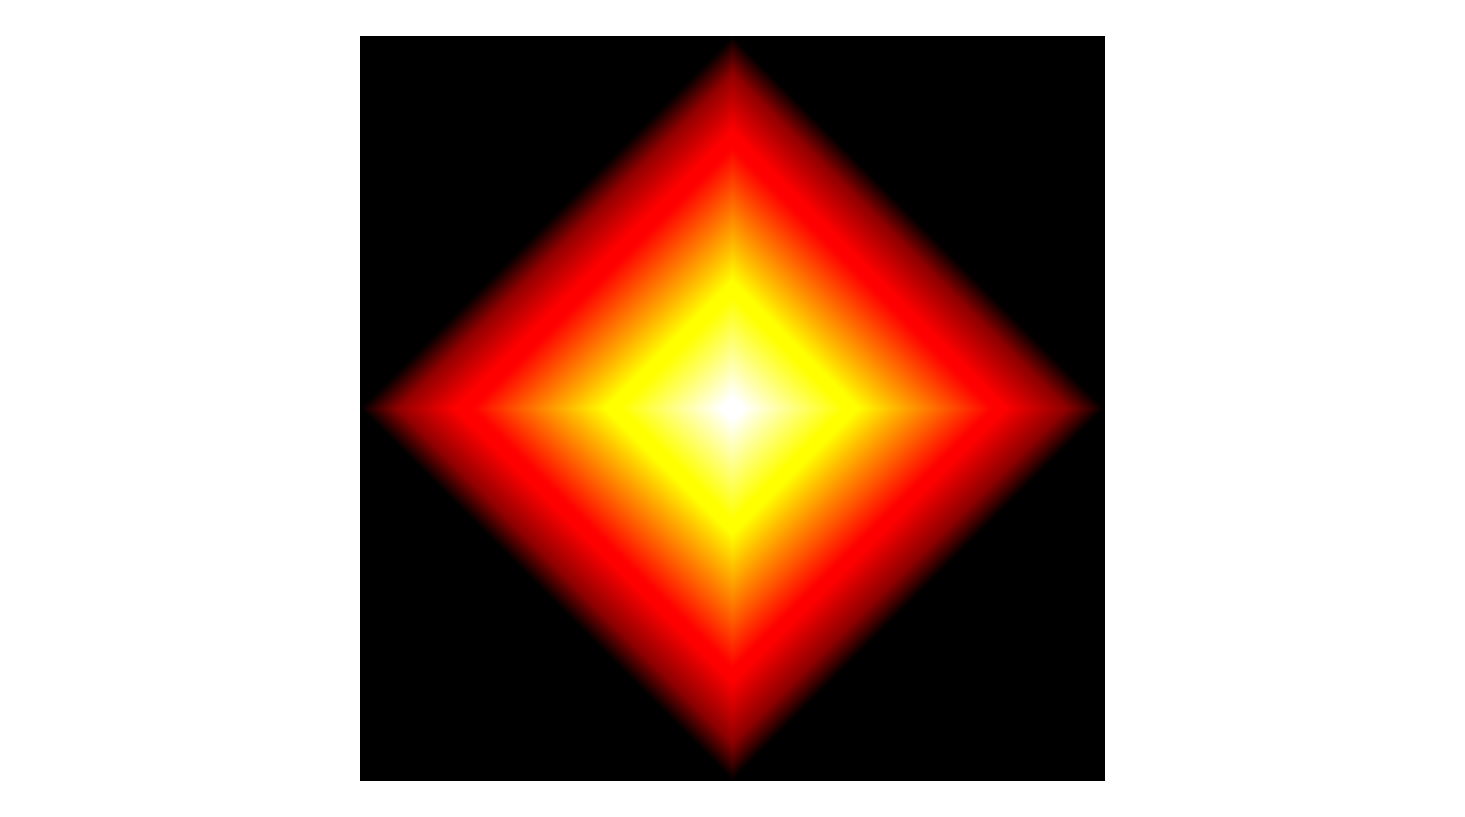
\includegraphics[width=\linewidth]
		{data/synthetic_meshes/square_tesselation_4tri_Dirac_delta_1_v13_f16_funcvals_0iter.png}
		\caption{$r=1$, $c=0$}\label{fig:sq2.b}
	\end{subfigure}
	\begin{subfigure}[b]{0.32\linewidth}
		
\includegraphics[width=\linewidth]
		{data/synthetic_meshes/square_tesselation_4tri_Dirac_delta_1_v13_f16_funcvals_1iter.png}
		\caption{$r=1$, $c=1$}\label{fig:sq2.c}
	\end{subfigure}

	\bigskip
	\begin{subfigure}[b]{0.32\linewidth}
		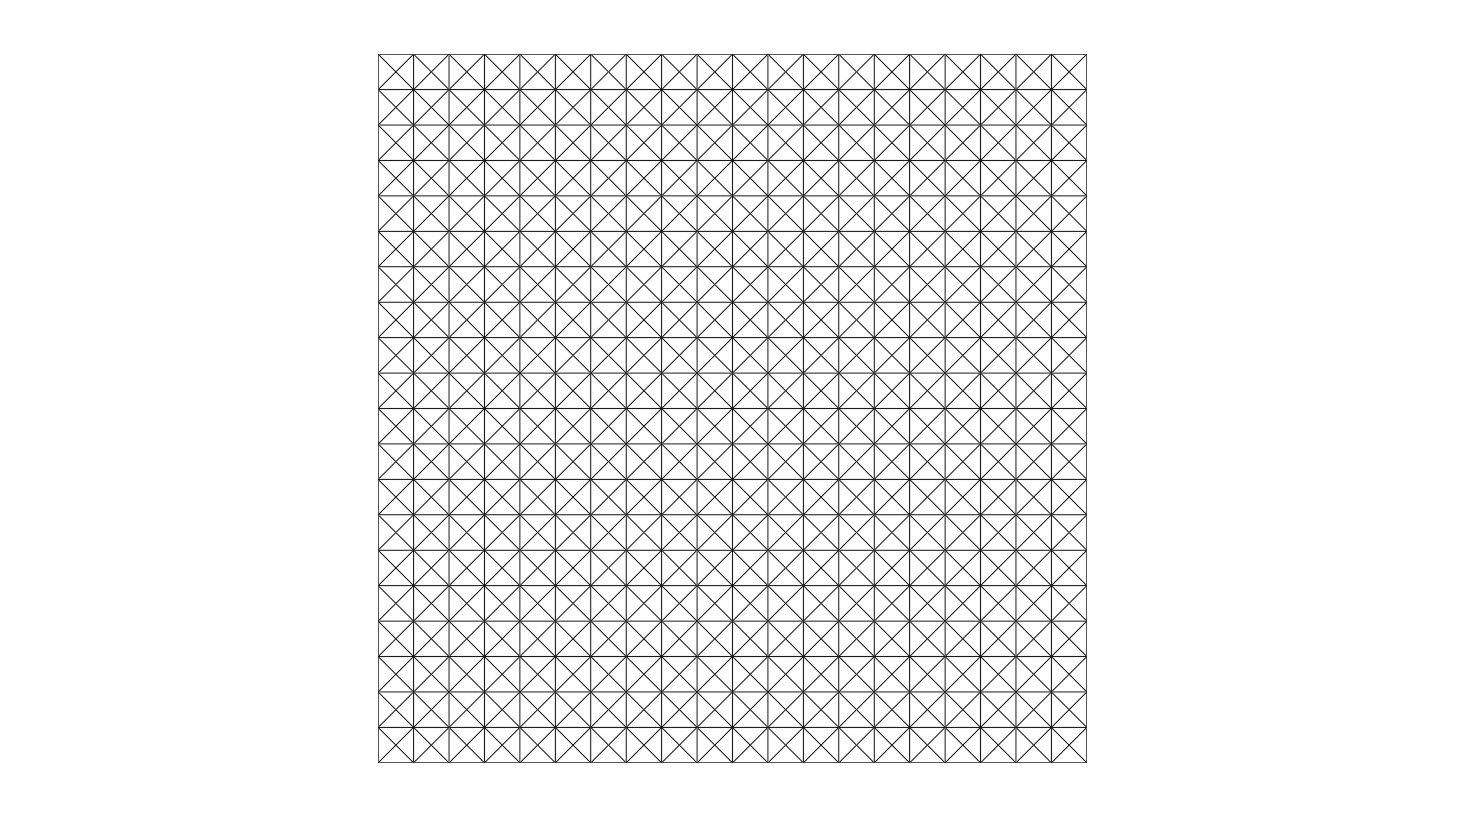
\includegraphics[width=\linewidth]
		{data/synthetic_meshes/square_tesselation_4tri_Dirac_delta_10_v841_f1600_wireframe.png}
		\caption{$r=10$, wireframe}\label{fig:sq2.d}
	\end{subfigure}
	\begin{subfigure}[b]{0.32\linewidth}
		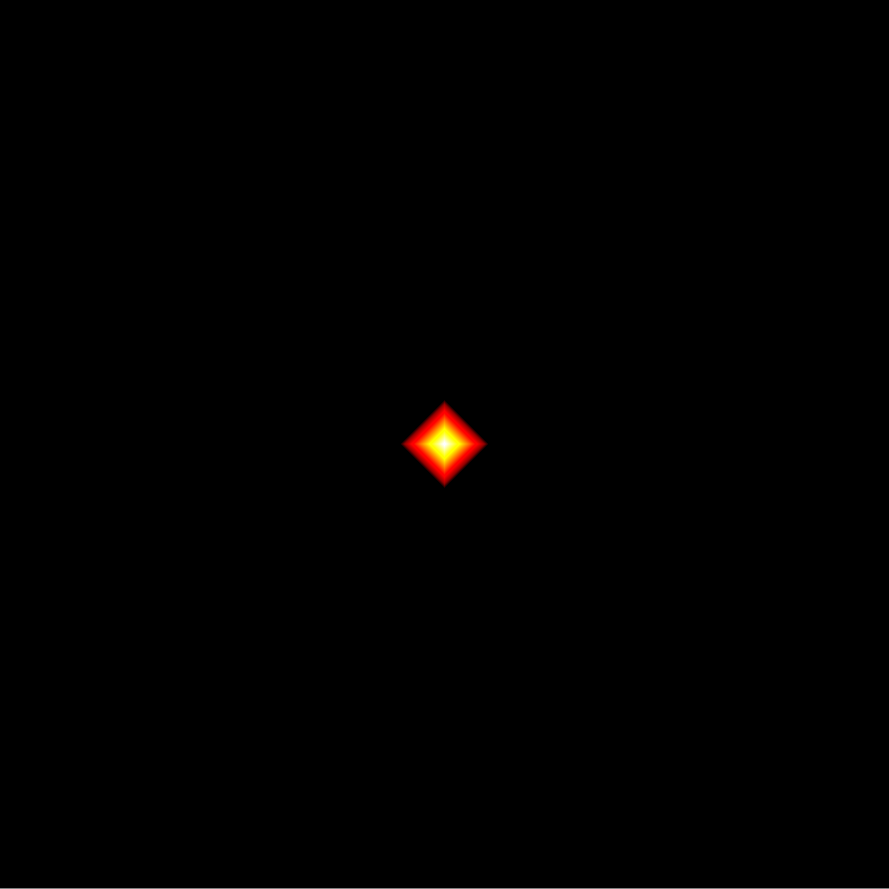
\includegraphics[width=\linewidth]
		{data/synthetic_meshes/square_tesselation_4tri_Dirac_delta_10_v841_f1600_funcvals_0iter.png}
		\caption{$r=10$, $c=0$}\label{fig:sq2.e}
	\end{subfigure}
	\begin{subfigure}[b]{0.32\linewidth}
		
\includegraphics[width=\linewidth]
		{data/synthetic_meshes/square_tesselation_4tri_Dirac_delta_10_v841_f1600_funcvals_100iter.png}
		\caption{$r=10$, $c=100$}\label{fig:sq2.f}
	\end{subfigure}
	\caption[Six views, comparing two differently sized of quadirsected square tessellations]{Comparison of two differently sized quadirsected square tessellations, generated with parameters $r$ set to 1 and 10: (a) $r=1$ in wireframe (b) $r=1$ colored by function value before convolving the filter (c) $r=1$ colored by function value after convolving the filter once (d) $r=10$ in wireframe (e) $r=10$ colored by function value before convoving the filter \newline(f) $r=10$ colored by function value after convolving the filter 100 times.}
	\label{fig:sq2}
\end{figure}

}

%------------------------------------------------
\frame{\frametitle{Hexagonal Tessellations}
	\begin{figure}[ht]
	\begin{subfigure}[b]{0.32\linewidth}
		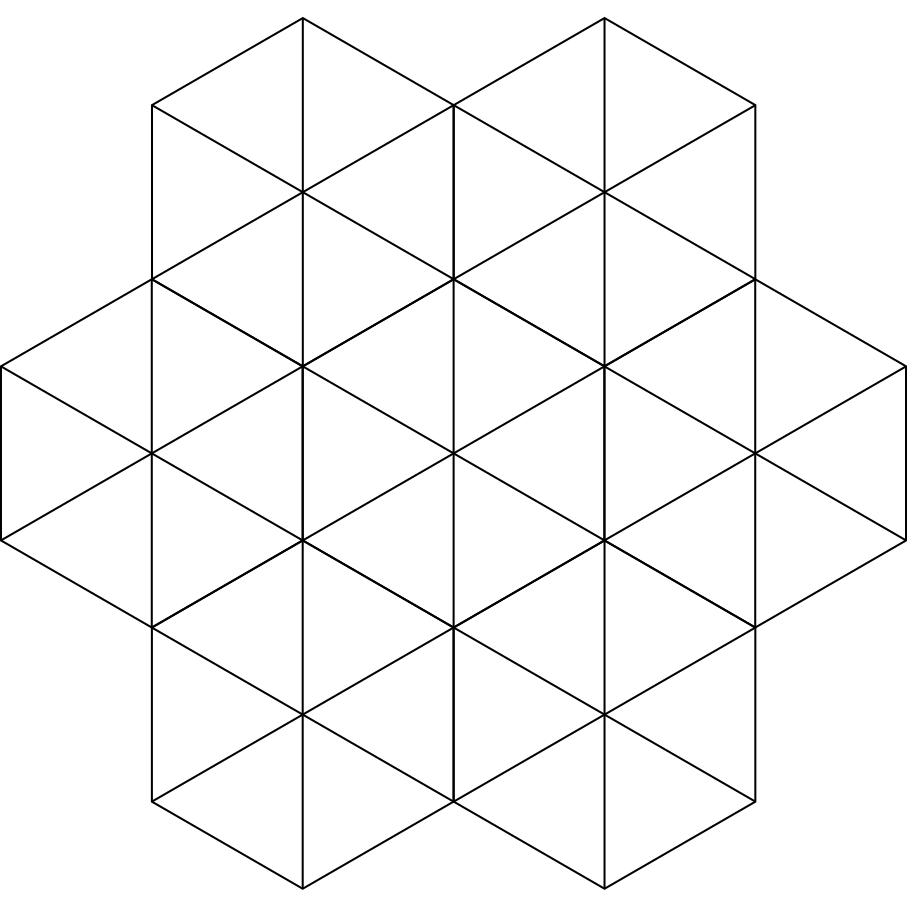
\includegraphics[width=\linewidth]
		{data/synthetic_meshes/hexagonal_tessellation_Dirac_delta_1_v31_f42_wireframe.png}
		\caption{$r=1$, wireframe}\label{fig:hex.a}
	\end{subfigure}
	\begin{subfigure}[b]{0.32\linewidth}
		
\includegraphics[width=\linewidth]
		{data/synthetic_meshes/hexagonal_tessellation_Dirac_delta_1_v31_f42_funcvals_0iter_crop.png}
		\caption{$r=1$, $c=0$}\label{fig:hex.b}
	\end{subfigure}
	\begin{subfigure}[b]{0.32\linewidth}
		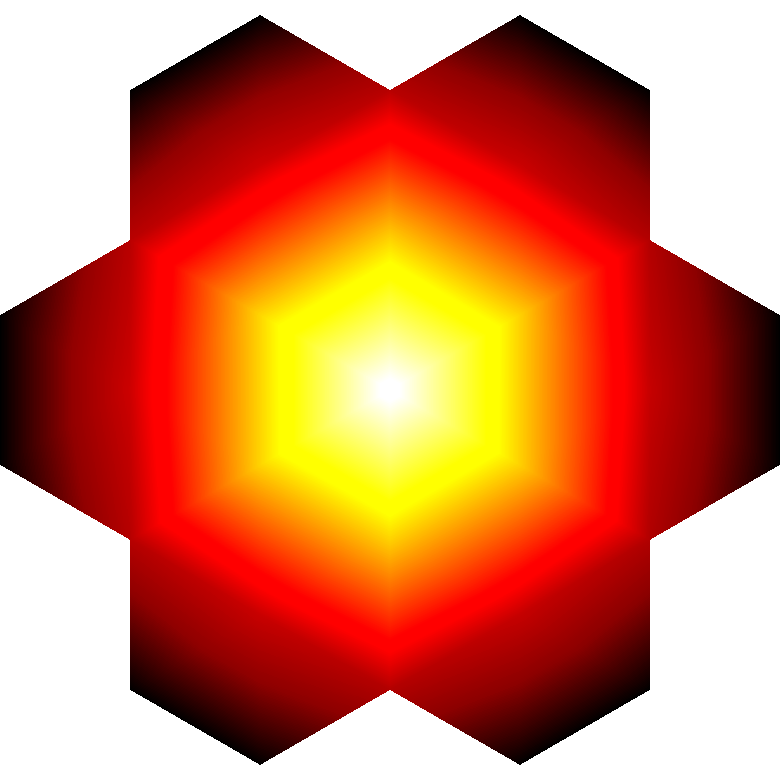
\includegraphics[width=\linewidth]
		{data/synthetic_meshes/hexagonal_tessellation_Dirac_delta_1_v31_f42_funcvals_2iter_crop.png}
		\caption{$r=1$, $c=2$}\label{fig:hex.c}
	\end{subfigure}

	\begin{subfigure}[b]{0.32\linewidth}
		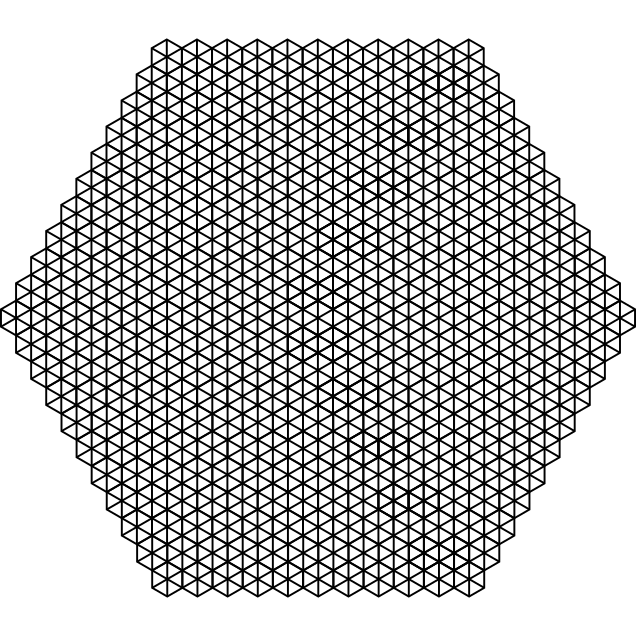
\includegraphics[width=\linewidth]
		{data/synthetic_meshes/hexagonal_tessellation_Dirac_delta_10_v1057_f1986_wireframe.png}
		\caption{$r=10$, wireframe}\label{fig:hex.d}
	\end{subfigure}
	\begin{subfigure}[b]{0.32\linewidth}
		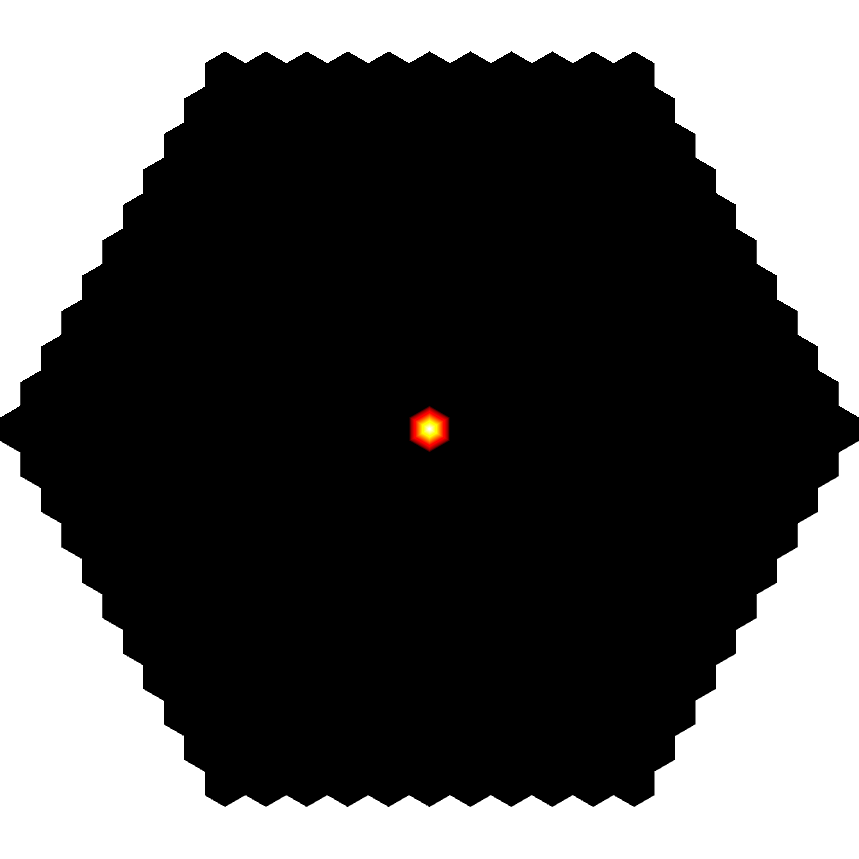
\includegraphics[width=\linewidth]
		{data/synthetic_meshes/hexagonal_tessellation_Dirac_delta_10_v1057_f1986_funcvals_0iter_crop.png}
		\caption{$r=10$, $c=0$}\label{fig:hex.e}
	\end{subfigure}
	\begin{subfigure}[b]{0.32\linewidth}
		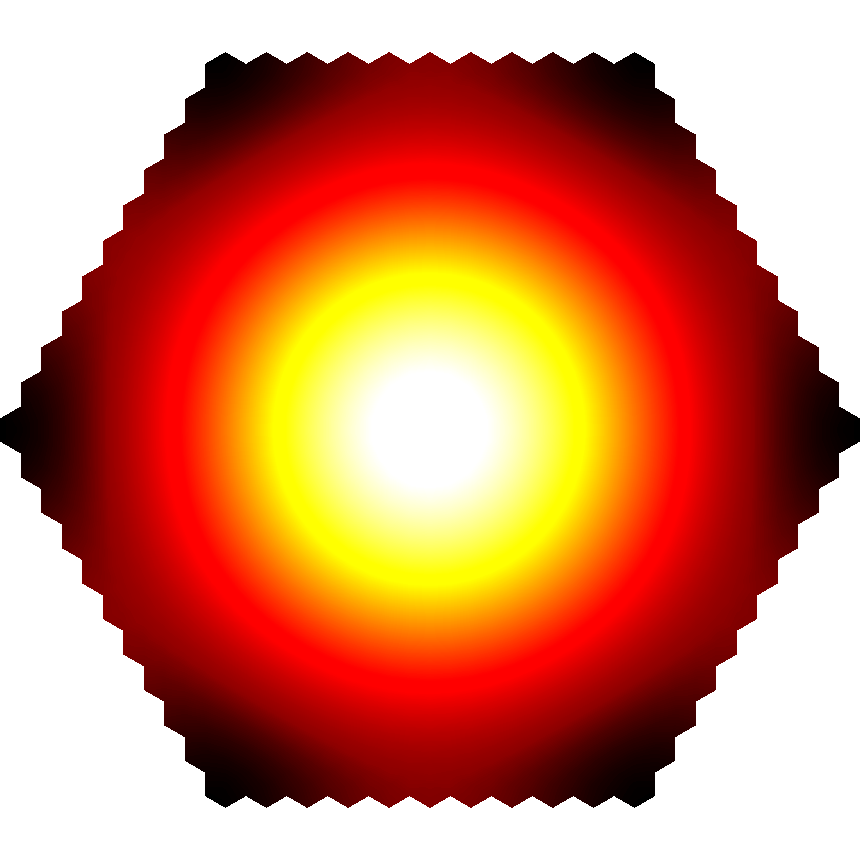
\includegraphics[width=\linewidth]
		{data/synthetic_meshes/hexagonal_tessellation_Dirac_delta_10_v1057_f1986_funcvals_200iter_crop.png}
		\caption{$r=10$, $c=200$}\label{fig:hex.f}
	\end{subfigure}
	\caption[Six Views Comparing Hexagonal Tessellations]{Comparison of two differently-sized, hexagonal tessellations, generated with parameters $r$ set to 1 and 10. (a) $r=1$ in wireframe, (b) $r=1$ colored by function value before convolving the filter, (c) $r=1$ colored by function value after convolving the filter once, (d) $r=10$ in wireframe, (e) $r=10$ colored by function value before convoving the filter, and (f) $r=10$ colored by function value after convolving the filter 200 times.}
	\label{fig:hex}
\end{figure}

}

%------------------------------------------------
\frame{\frametitle{Random Triangulated Discs}
	\begin{figure}[ht]
	\begin{subfigure}[b]{0.32\linewidth}
		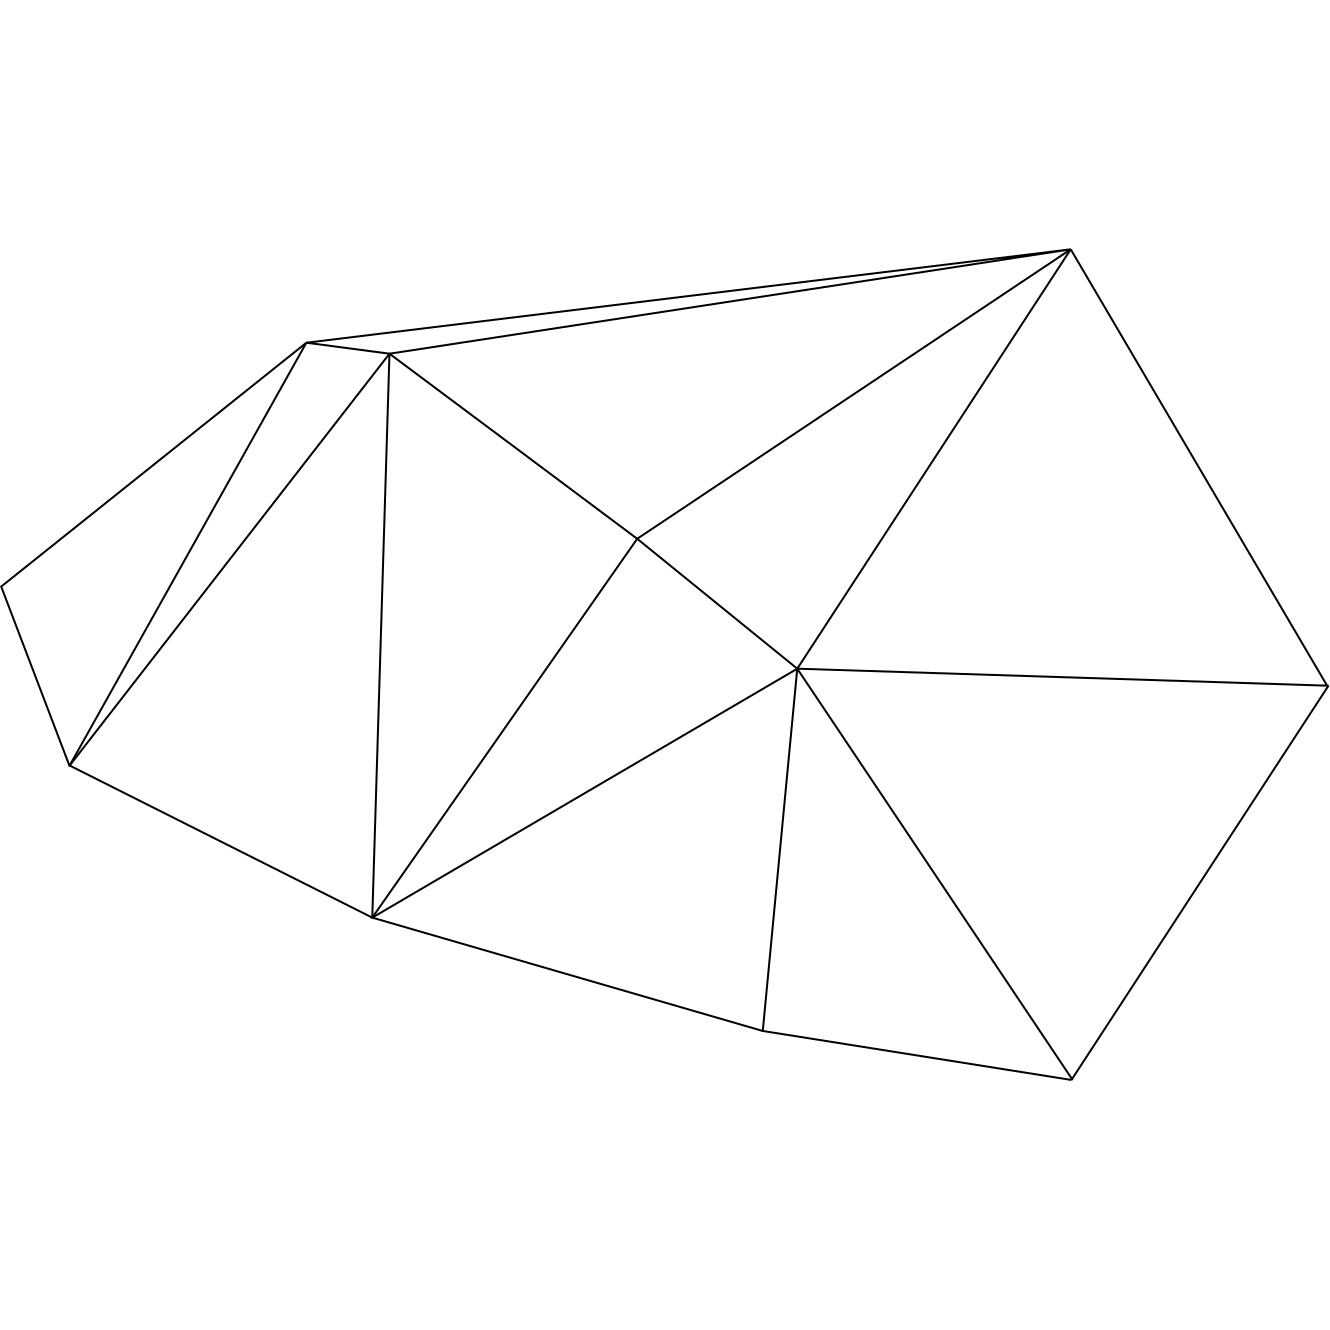
\includegraphics[width=\linewidth]
		{data/synthetic_meshes/random_circle_tessellation_Dirac_delta_1_v11_f12_wireframe.png}
		\caption{$r=1$, $p=11$, wireframe}\label{fig:rcirc.a}
	\end{subfigure}
	\begin{subfigure}[b]{0.32\linewidth}
		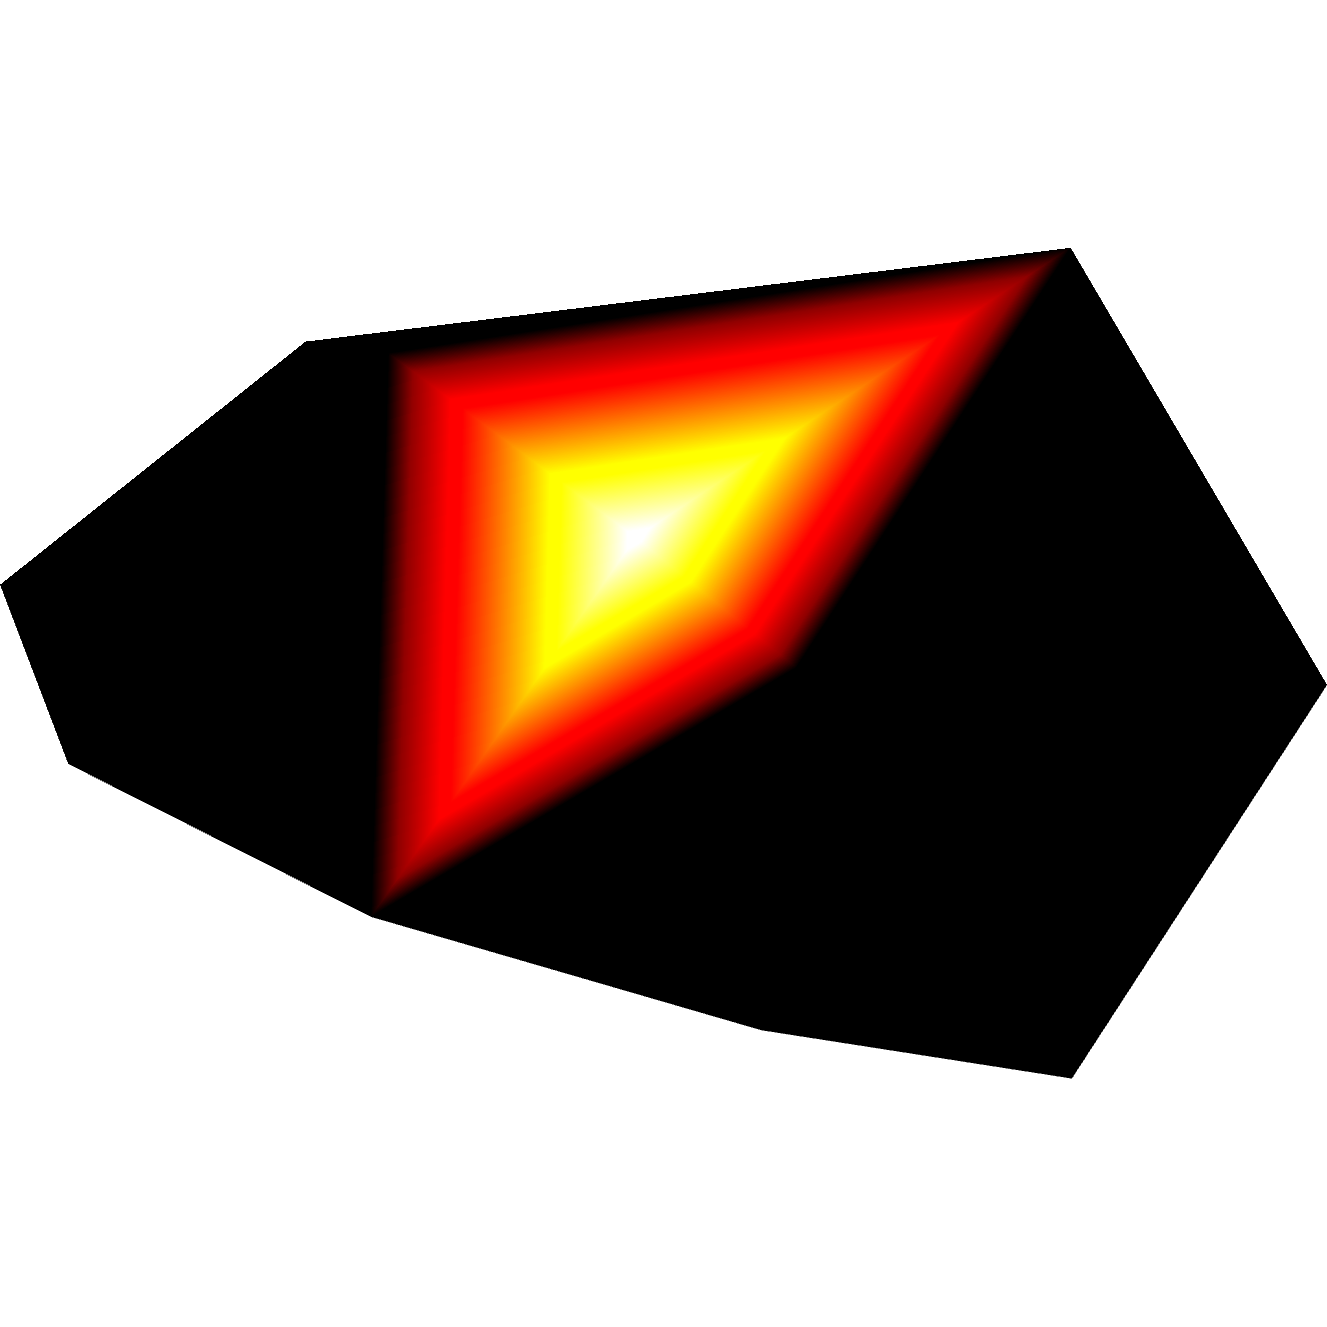
\includegraphics[width=\linewidth]
		{data/synthetic_meshes/random_circle_tessellation_Dirac_delta_1_v11_f12_funcvals_0iter.png}
		\caption{$r=1$, $p=11$, $c=0$}\label{fig:rcirc.c}
	\end{subfigure}
	\begin{subfigure}[b]{0.32\linewidth}
		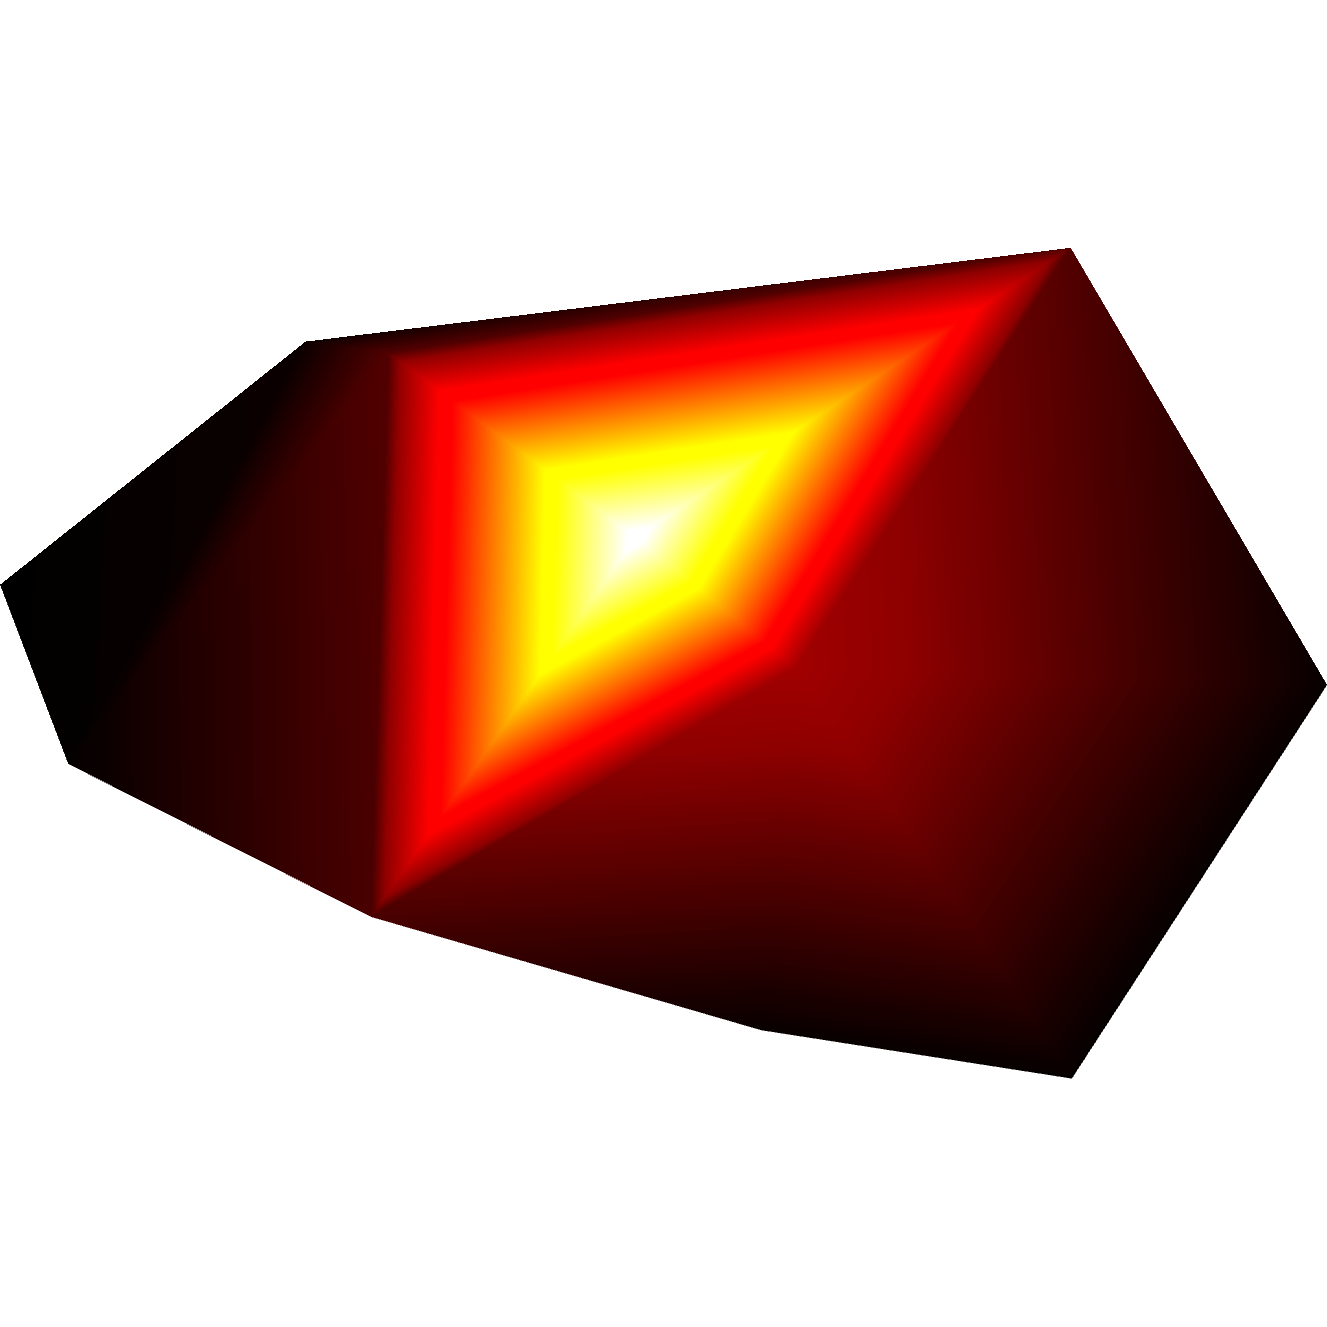
\includegraphics[width=\linewidth,]
		{data/synthetic_meshes/random_circle_tessellation_Dirac_delta_1_v11_f12_funcvals_2iter.png}
		\caption{$r=1$, $p=11$, $c=2$}\label{fig:rcirc.e}
	\end{subfigure}

	\bigskip
	\begin{subfigure}[b]{0.32\linewidth}
		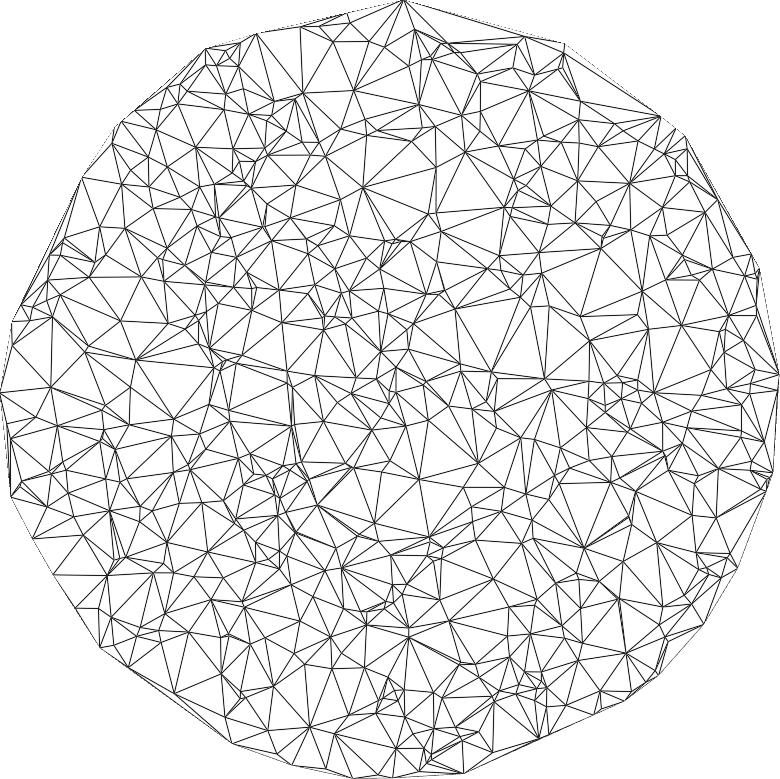
\includegraphics[width=\linewidth]
		{data/synthetic_meshes/random_circle_tessellation_Dirac_delta_10_v641_f1252_wireframe.png}
		\caption{$r=10$, $p=641$, wireframe}\label{fig:rcirc.b}
	\end{subfigure}
	\begin{subfigure}[b]{0.32\linewidth}
		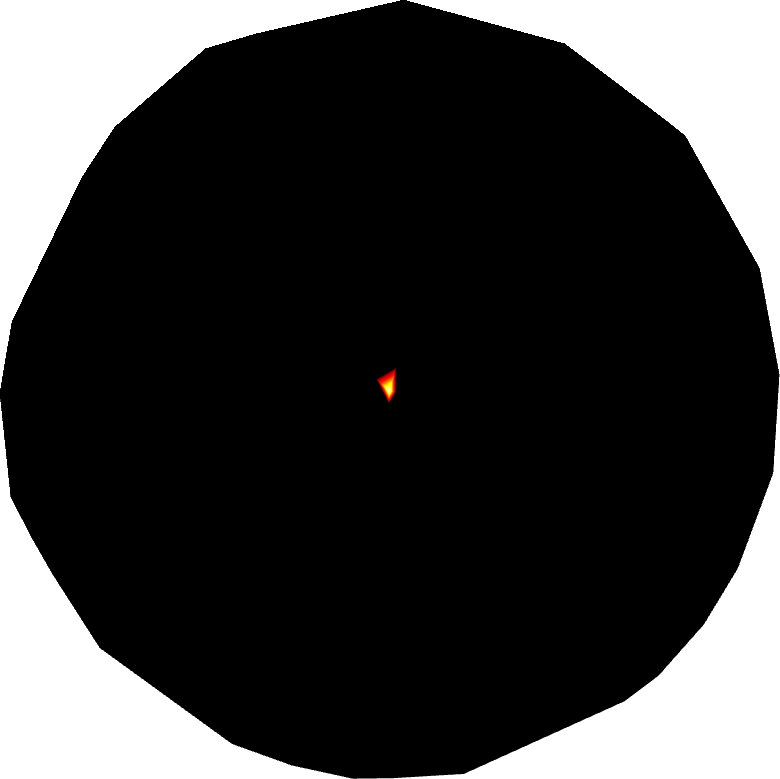
\includegraphics[width=\linewidth]
		{data/synthetic_meshes/random_circle_tessellation_Dirac_delta_10_v641_f1252_funcvals_0iter.png}
		\caption{$r=10$, $p=641$, $c=0$}\label{fig:rcirc.d}
	\end{subfigure}
	\begin{subfigure}[b]{0.32\linewidth}
		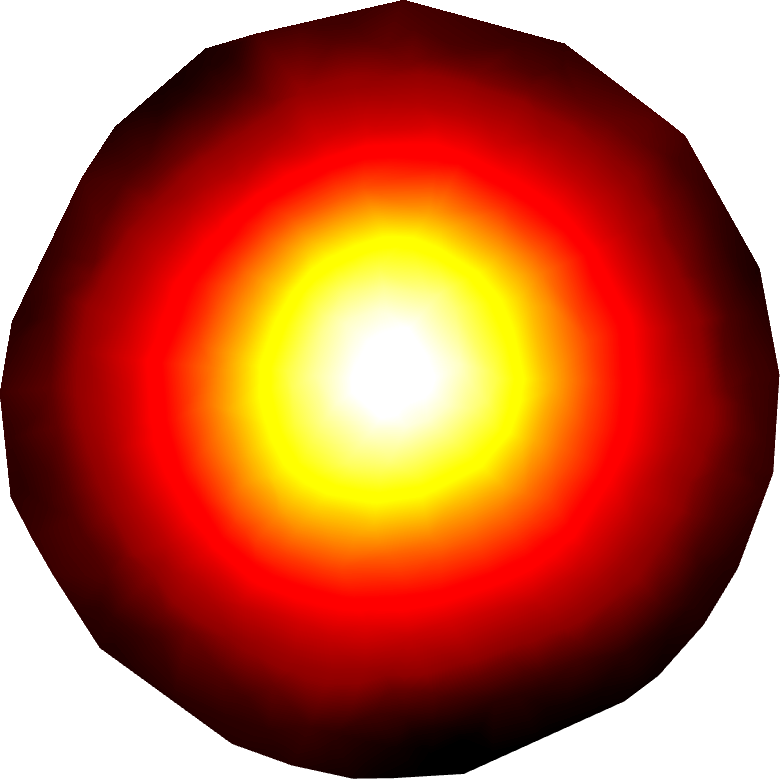
\includegraphics[width=\linewidth]
		{data/synthetic_meshes/random_circle_tessellation_Dirac_delta_10_v641_f1252_funcvals_10000iter.png}
		\caption{$r=10$, $p=641$, $c=10^4$}\label{fig:rcirc.f}
	\end{subfigure}
	\caption[Six views, comparing two differently sized, random triangulated discs]{Comparison of two differently sized, random triangulated discs, generated with parameters $r$ set to 1 and 10, and parameters $p$ set to 11 and 641: (a) $r=1$, $p=11$ in wireframe (b) $r=1$, $p=11$ colored by function value before convolving the filter (c) $r=1$, $p=11$ colored by function value after convolving the filter twice (d) $r=10$, $p=641$ in wireframe (e) $r=10$, $p=641$ colored by function value before convoving the filter (f) $r=10$, $p=641$ colored by function value after convolving the filter 10,000 times.}
	\label{fig:rdisc}
\end{figure}


}


%================================================
\subsection{Filter Response On Acquired Data}

%------------------------------------------------
\frame{\frametitle{The University of Heidelberg Seal}
	\begin{figure}[ht]
	\begin{subfigure}[b]{0.32\linewidth}
		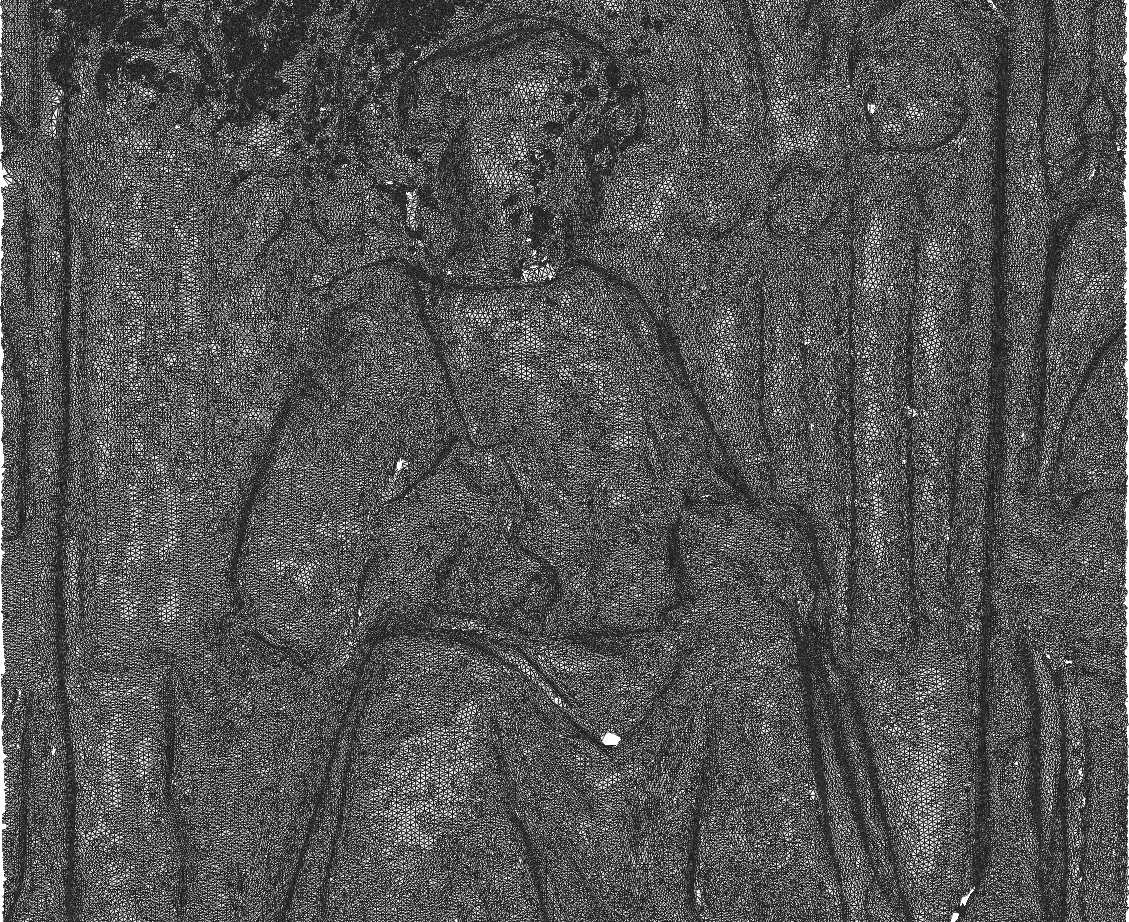
\includegraphics[width=\linewidth]{data/acquired_meshes/unisiegel_wireframe.png}
		\caption{wireframe}\label{fig:unisiegel.a}
	\end{subfigure}
	\begin{subfigure}[b]{0.32\linewidth}
		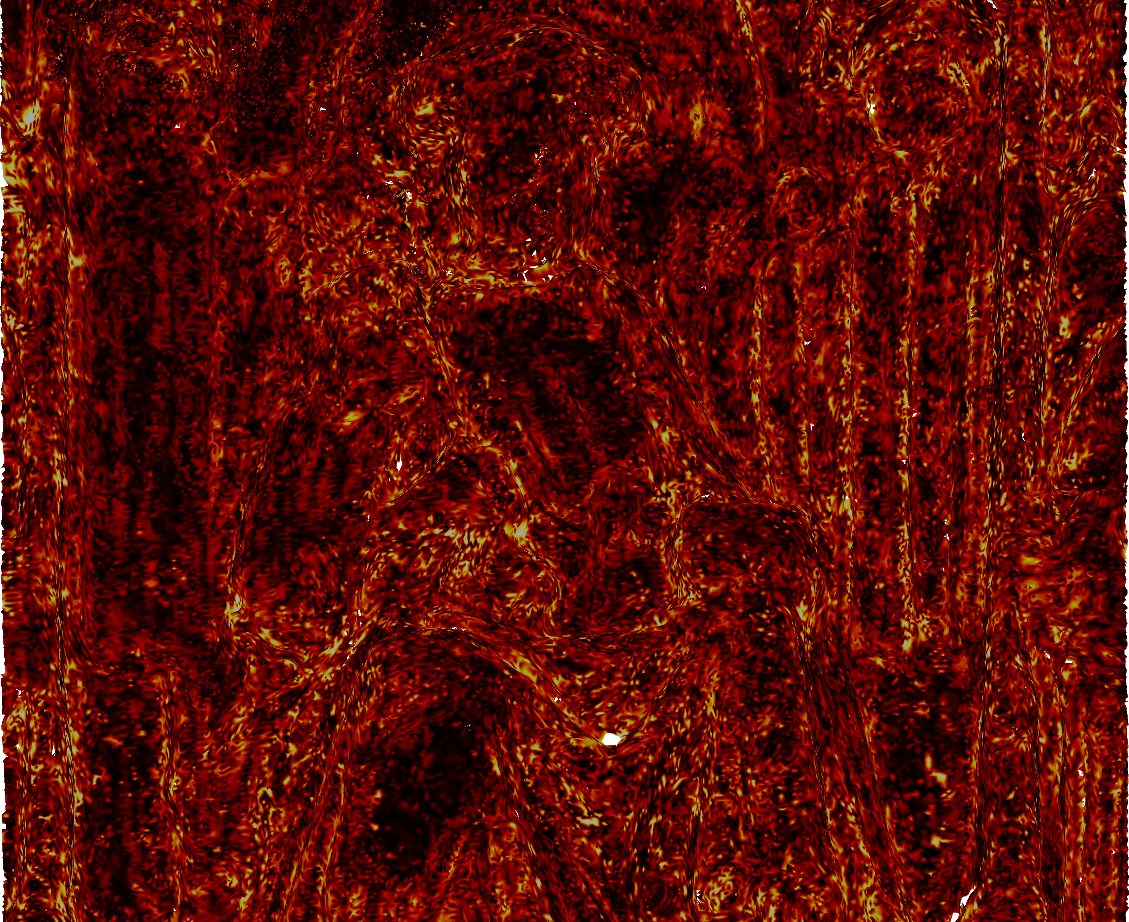
\includegraphics[width=\linewidth]{data/acquired_meshes/unisiegel_0iter.png}
		\caption{$c=0$}\label{fig:unisiegel.b}
	\end{subfigure}
	\begin{subfigure}[b]{0.32\linewidth}
		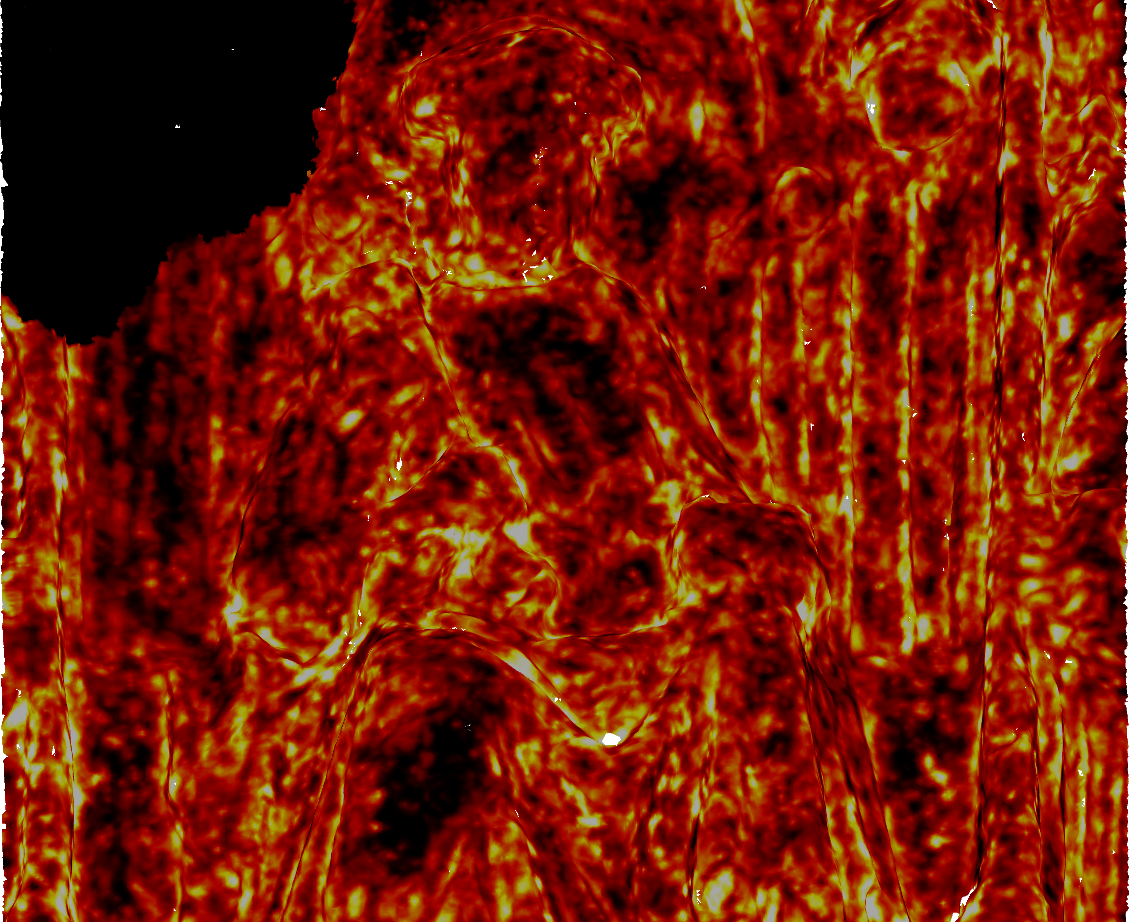
\includegraphics[width=\linewidth]{data/acquired_meshes/unisiegel_100iter.png}
		\caption{$c=100$}\label{fig:unisiegel.c}
	\end{subfigure}
	\caption[Three views of the Univeristy of Heidelberg Seal]{Three views of the Univeristy of Heidelberg seal (a) in wireframe, (b) colored by \gls{tMSIIf} value before convolving the filter, (c) colored by function value after convolving the filter 100 times.}
	\label{fig:unisiegel}
\end{figure}

}

%------------------------------------------------
\frame{\frametitle{A flat surface from ILATO}
	\begin{figure}[ht]
	\begin{subfigure}[b]{0.49\linewidth}
		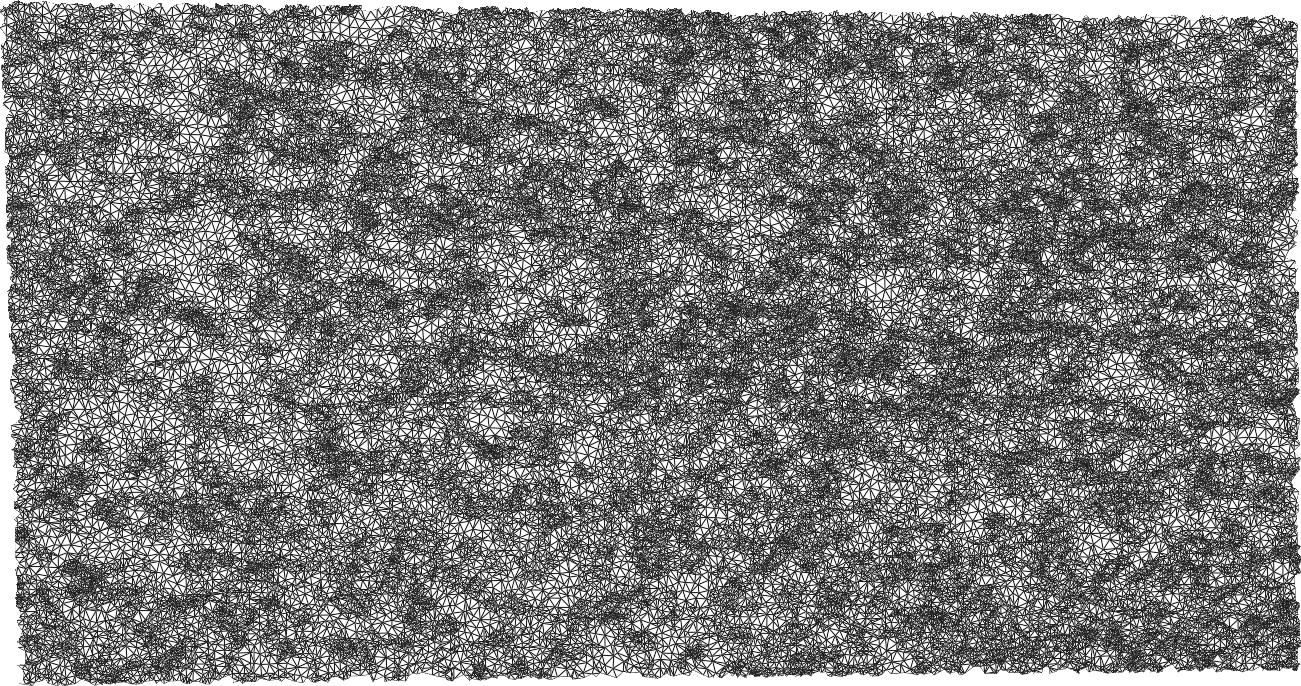
\includegraphics[width=\linewidth]
		{data/acquired_meshes/ILATO_1A_SM2066-HE5-60_070214_merged_GMO_r1_n4_v256_wireframe.png}
		\caption{wireframe}\label{ILATO:bun.a}
	\end{subfigure}
	\begin{subfigure}[b]{0.49\linewidth}
		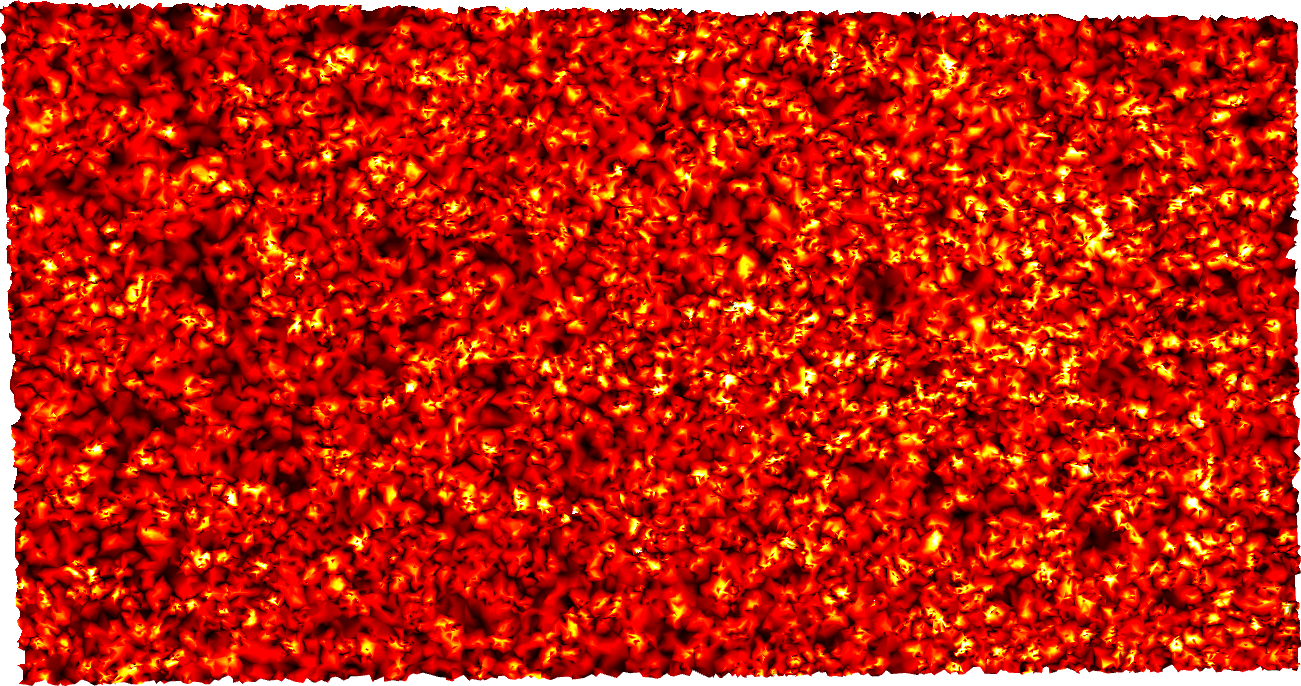
\includegraphics[width=\linewidth]
		{data/acquired_meshes/ILATO_1A_SM2066-HE5-60_070214_merged_GMO_r1_n4_v256_funcvals_0iter.png}
		\caption{$c=0$}\label{fig:buILATOn.b}
	\end{subfigure}

	\bigskip
	\begin{subfigure}[b]{0.49\linewidth}
		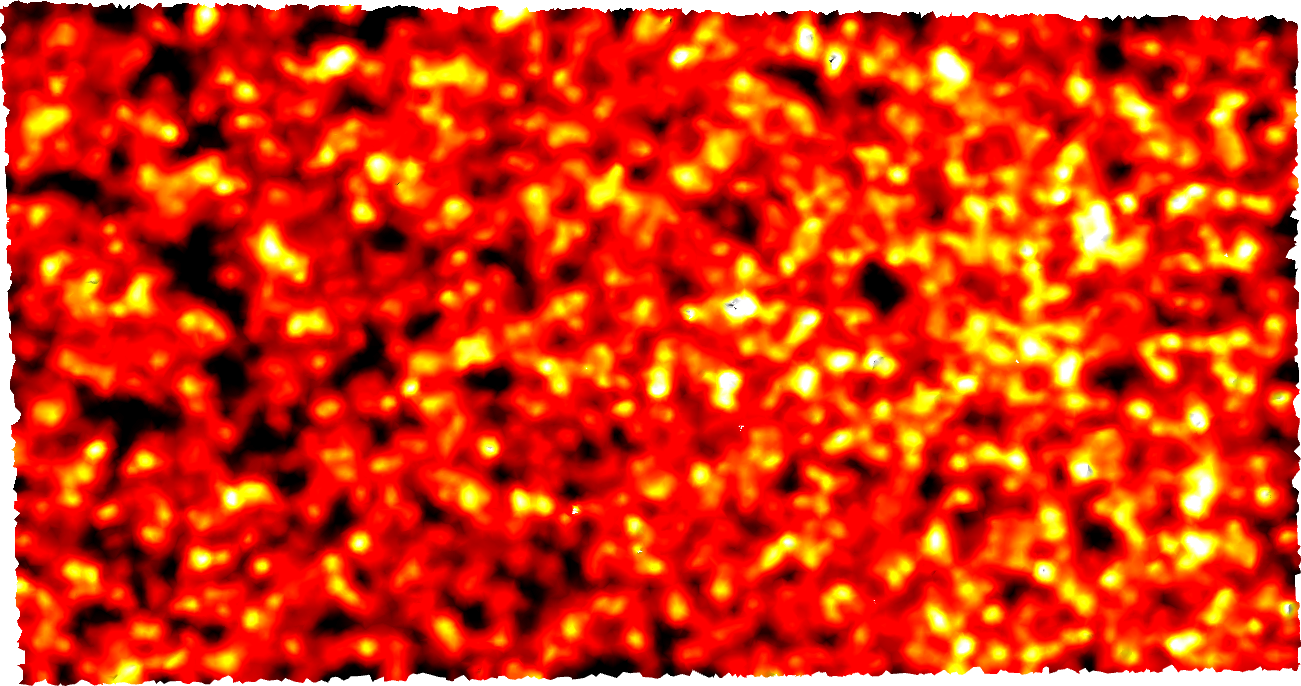
\includegraphics[width=\linewidth]
		{data/acquired_meshes/ILATO_1A_SM2066-HE5-60_070214_merged_GMO_r1_n4_v256_funcvals_1000iter.png}
		\caption{$c=1000$}\label{fig:ILATO.c}
	\end{subfigure}
	\begin{subfigure}[b]{0.49\linewidth}
		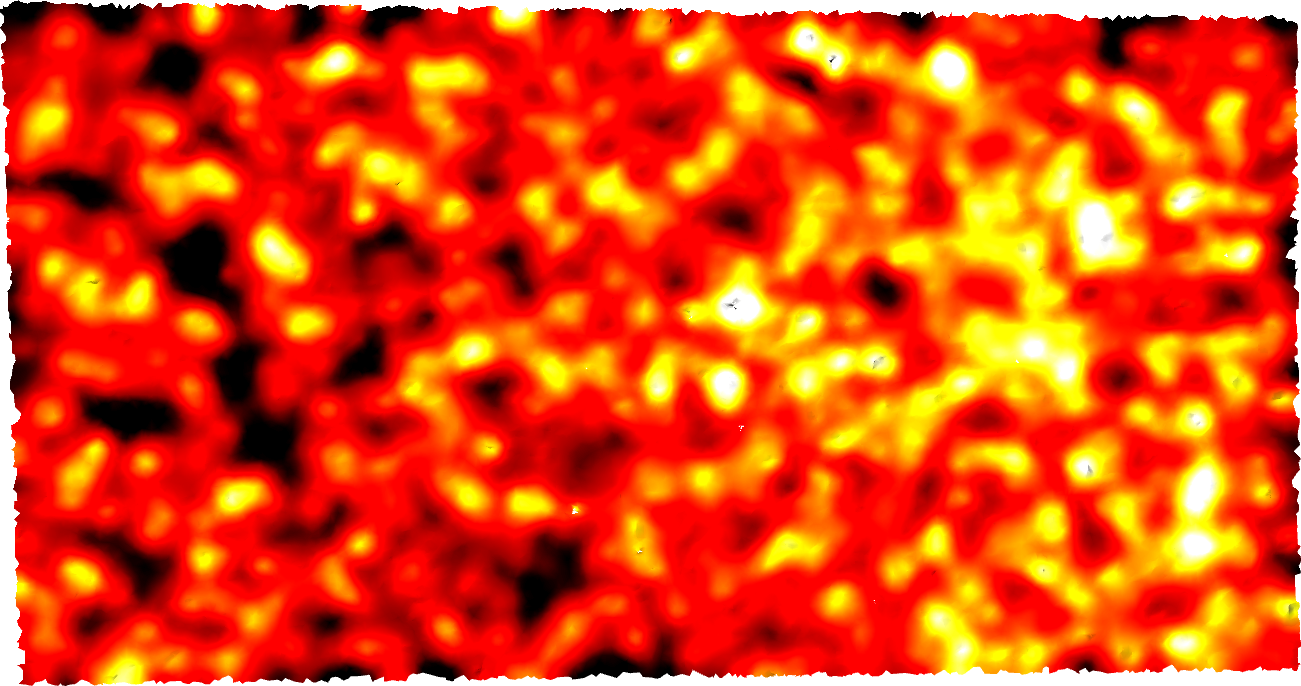
\includegraphics[width=\linewidth]
		{data/acquired_meshes/ILATO_1A_SM2066-HE5-60_070214_merged_GMO_r1_n4_v256_funcvals_3000iter.png}
		\caption{$c=3000$}\label{fig:ILATO.d}
	\end{subfigure}
	\caption[Four Views of the Flat Surface from ILATO]{Four views of a flat surface (a) in wireframe (b) colored by MSII function value before convolving the filter (c) colored by function value after convolving the filter 1,000 times (c) and after 3,000 times.}
	\label{fig:ILATO}
\end{figure}

}

%------------------------------------------------
\frame{\frametitle{The Stanford Bunny}
	\begin{figure}[ht]
	\begin{subfigure}[b]{0.32\linewidth}
		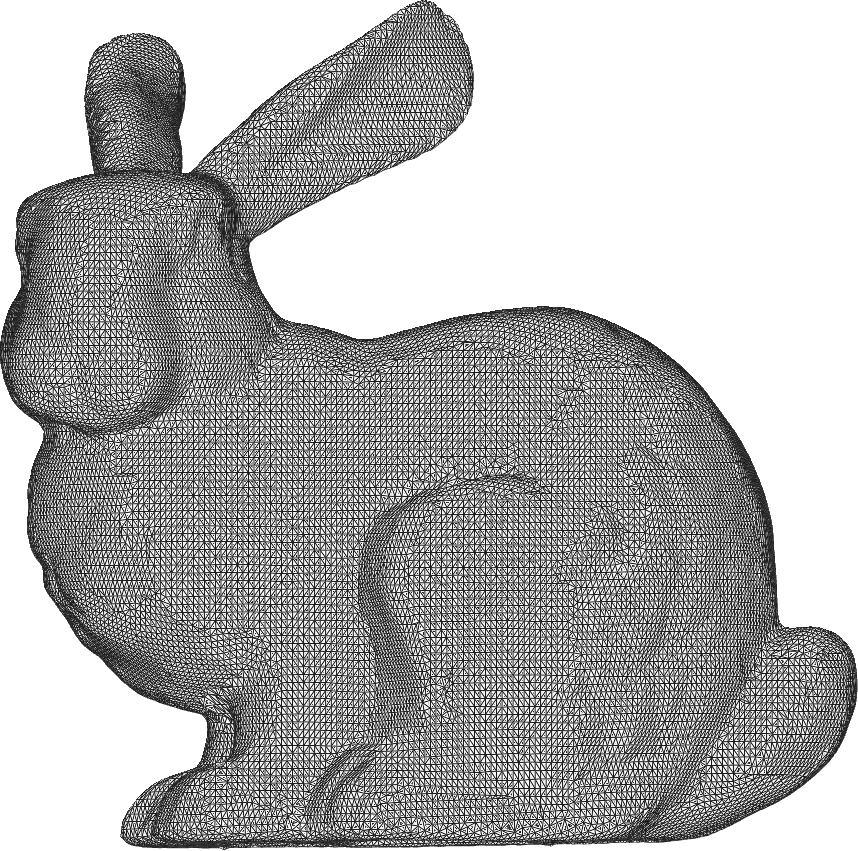
\includegraphics[width=\linewidth]
		{data/acquired_meshes/bun_zipper_edited_r1_n4_v256_wireframe.png}
		\caption{wireframe}\label{fig:bun.a}
	\end{subfigure}
	\begin{subfigure}[b]{0.32\linewidth}
		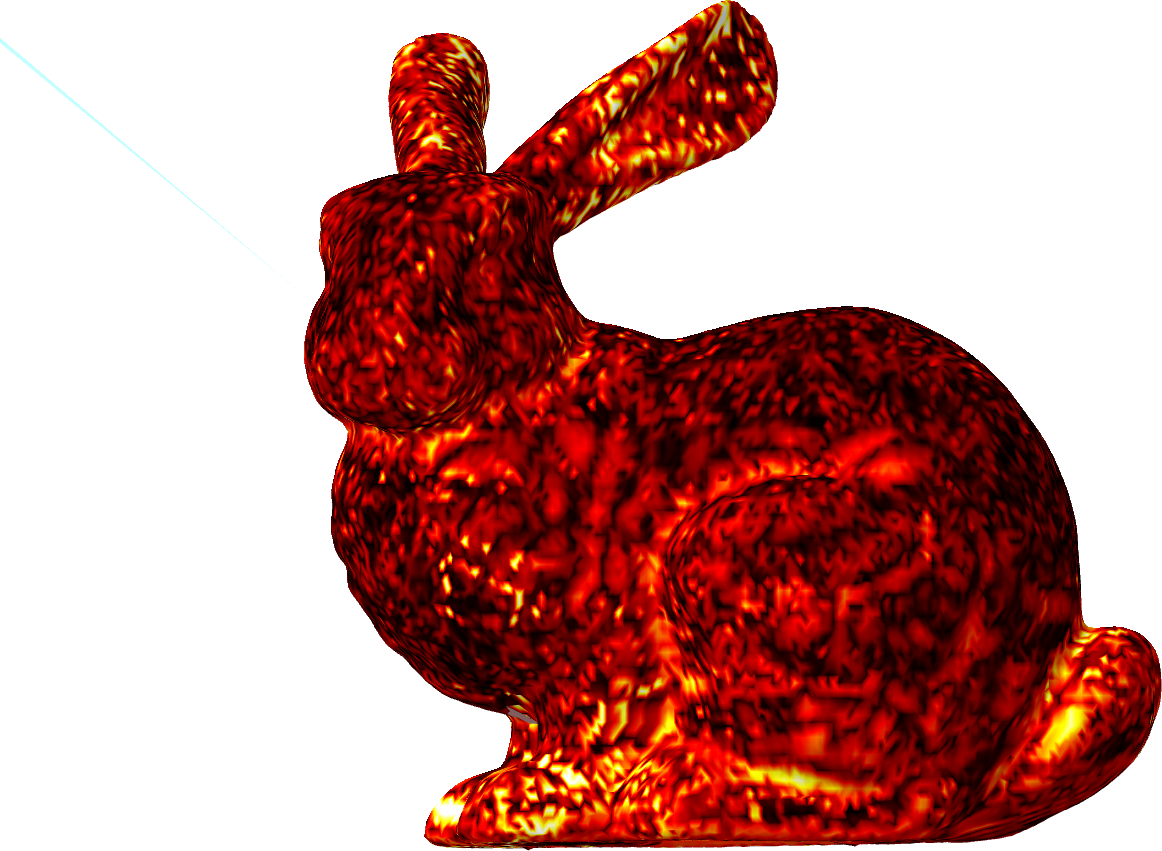
\includegraphics[width=\linewidth]
		{data/acquired_meshes/bun_zipper_edited_r1_n4_v256_funcvals_0iter.png}
		\caption{$c=0$}\label{fig:bun.b}
	\end{subfigure}
	\begin{subfigure}[b]{0.32\linewidth}
		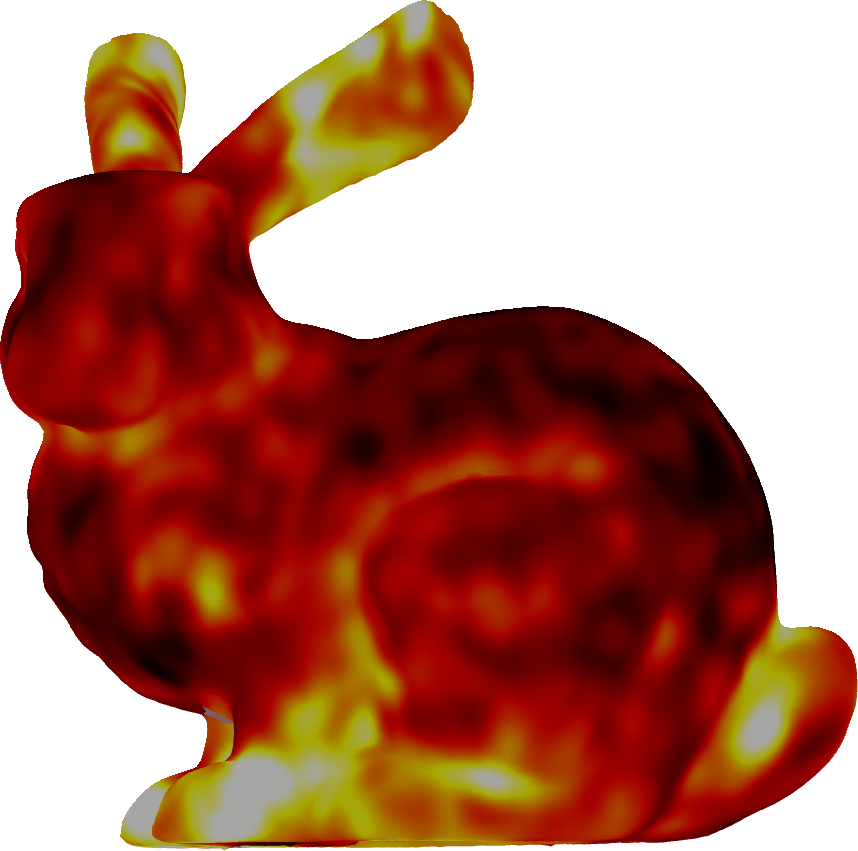
\includegraphics[width=\linewidth]
		{data/acquired_meshes/bun_zipper_edited_r1_n4_v256_funcvals_100iter.png}
		\caption{$c=100$}\label{fig:bun.c}
	\end{subfigure}
	\caption[Three Views of the Stanford Bunny]{Three views of the Stanford Bunny (a) in wireframe, (b) colored by \gls{tMSIIf} value before convolving the filter, and (c) colored by function value after convolving the filter 100 times.}
	\label{fig:bun}
\end{figure}

}




%================================================
\subsection{Convolving with a GPGPU}

%------------------------------------------------
\frame{\frametitle{Evaluation and Analysis of Parallel Algorithms}

\begin{align*}
	\mathit{T_s}(\hat{n}) &= \text{The optimal sequential execution time} \\
	\mathit{T_{\rho}}(\hat{n},\,\rho) &= \text{Parallel runtime}
\end{align*}

which can then be used to define the three essential metrics:

\begin{align*}
	\text{Speedup:}\quad&\mathit{S}(\hat{n},\,\rho) = \frac{\mathit{T_s}(\hat{n})}{\mathit{T_{\rho}}(\hat{n},\,\rho)} \\
	\text{Costs}:\quad&\mathit{C}(\hat{n},\,\rho) =\rho\cdot\mathit{T_{\rho}}(\hat{n},\,\rho) \\
	\text{Efficiency}:\quad&\mathit{E}(\hat{n},\,\rho) = \frac{\mathit{T_s}(\hat{n})}{\mathit{C}(\hat{n},\,\rho)} = \frac{\mathit{S}(\hat{n},\,\rho)}{\rho}
\end{align*}
}

%------------------------------------------------
\frame{\frametitle{Amdahl's law and the Degree of Parallelism}
Also important is the notion of an algorithm's ``degree of parallelism'', which is the maximum number of operations that can be executed in parallel, a principle central to Amdahl's law which is defined as, when given a constant problem size $\hat{n}_{fixed}$, and an algorithm's degree of parallelism $q$,

\begin{equation*}
	\lim_{\rho \to \infty} \mathit{S}(\hat{n}_{fixed},\,\rho) = 1 / q
\end{equation*}

This leads to the conclusion that one can not simply add more processors in order to gain appreciable speedup, but instead that relies heavily on processor counts which grow in relation to problem sizes, and the degree of parallelism, which itself relies on the underlying nature of the serial algorithm and the artful design of the parallel algorithm.
}

%------------------------------------------------
\frame{\frametitle{Compute Times per Experiment for increasing Convolution Counts}
\begin{figure}[ht]
\includegraphics[width=1.0\linewidth,height=1.0\textheight,keepaspectratio]
	{figures/computeTimesLinespoints.png}
	\caption[Compute Times per Experiment for increasing Convolution Counts]{Compute times per experiment, for increasing numbers of convolutions of \fors{t}, onto acquired and synthetic \tdd{} of varying sizes. Combinations involving the smallest mesh sizes are colored red, the largest mesh sizes in blue, with all others scaled in between. The experiments involving acquired \tdd{} are specially marked with squares for the flat surface mesh, and circles for the university seal.

\vspace*{\baselineskip}
\scriptsize† The experiment codes used correspond to: the system, T for the desktop or M for the laptop; the algorithm variant, P for parallel or S for serial; the mesh being processed, BS for bisected-square, HT for hexagonal tessellation, US for university seal, and FS for the flat surface; and finally, the count of points comprising the mesh.}
	\label{fig:computeTimesLP}
\end{figure}
}

%------------------------------------------------
\frame{\frametitle{Compute Times Scatter Plot}
\begin{figure}[ht]
	\includegraphics[width=\linewidth]{figures/computeTimesScatter.png}
	\caption[Compute Times Scatter Plot]{A plot of the total compute times of each experiment as the area of a circle, given different hardware configurations. Each is then plotted for each combination of mesh size measured in point counts, and the number of convolutions of \Fors{t}. Blue circles indicate the serial variant computed with a \gls{CPU}, and a red circle indicates the parallel variant was computed on a \gls{GPGPU}.

\vspace*{\baselineskip}
\scriptsize† See Figure\ref{fig:computeTimesLP} for an explanation of the experiment codes.}
	\label{fig:computeTimesS}
\end{figure}
}

%------------------------------------------------
\frame{\frametitle{Speedup}
\begin{figure}[ht]
	\includegraphics[width=\linewidth]{figures/speedup.png}
	\caption[Speedup]{A graph of the \gls{speedup} obtained by convolving the parallel variant of \Fors{t} over meshes of different sizes. Lines in blue, increasing in saturation with the size of the mesh, are experiments run using the \gls{GPGPU} of laptop M with 768 \gls{CUDA} cores. Lines in red, increasing in saturation with the size of the mesh, are experiments run using the \gls{GPGPU}  of desktop T with 2,560 \gls{CUDA} cores. The experiments involving acquired \tdd{} are specially marked with squares for the flat surface mesh, and circles for the university seal.

\vspace*{\baselineskip}
\scriptsize† See Figure~\ref{fig:computeTimesLP} for an explanation of the experiment codes.}
	\label{fig:speedup}
\end{figure}
}

%------------------------------------------------
\frame{\frametitle{Efficiency}
\begin{figure}[ht]
	\includegraphics[width=\linewidth]{figures/efficiency.png}
	\caption[Efficiency]{A graph of the \gls{efficiency} obtained by convolving the parallel variant of \Fors{t} over meshes of different sizes. Lines in blue, increasing in saturation with the size of the mesh, are experiments run using the \gls{GPGPU} of laptop M with 768 \gls{CUDA} cores. Lines in red, increasing in saturation with the size of the mesh, are experiments run using the \gls{GPGPU} of desktop T with 2,560 \gls{CUDA} cores. The experiments involving acquired \tdd{} are specially marked with squares for the flat surface mesh and circles for the university seal.

\vspace*{\baselineskip}
\scriptsize† See Figure~\ref{fig:computeTimesLP} for an explanation of the experiment codes.}
	\label{fig:efficiency}
\end{figure}
}


%================================================
%================================================
\section[Conclusion]{Conclusion \& Outlook}

%------------------------------------------------
\frame{\frametitle{Conclusion}
	\begin{itemize}
		\item item 1
		\item item 1
		\item item 1
		\item item 1
		\item item 1
	\end{itemize}
}

%------------------------------------------------
\frame{\frametitle{Outlook}
	\begin{itemize}
		\item item 1
		\item item 1
		\item item 1
		\item item 1
		\item item 1
	\end{itemize}
}

%------------------------------------------------
\frame{\frametitle{Questions}
	
\includegraphics[width=.8\textwidth]{questions}
	\vspace*{-3.3cm}
	\begin{center}
		\begin{LARGE}
			\textbf{Questions}
		\end{LARGE}
	\end{center}
	\vspace*{2cm}
}

\end{document}
